% Standalone single-column preprint build aligned with the Study 3 preprint.
\documentclass[12pt]{article}

\usepackage[T1]{fontenc}
\usepackage[utf8]{inputenc}
\usepackage[margin=1in]{geometry}
\usepackage{setspace}
\usepackage[natbibapa]{apacite}
\usepackage[mathlines,switch]{lineno}
\usepackage[hidelinks]{hyperref}
\usepackage{url}
\usepackage[final,protrusion=true,expansion=false]{microtype}
\usepackage{caption}
\usepackage{graphicx}
\graphicspath{{figures/}}
\IfFileExists{wrapfig2.sty}{\usepackage{wrapfig2}}{\usepackage{wrapfig}}
\usepackage{amsmath,amssymb}
\usepackage{xcolor}
\usepackage{authblk}

\urlstyle{same}
\raggedbottom
\onehalfspacing
\setlength{\parskip}{0.35em}
\setlength{\parindent}{1.2em}
\setlength{\affilsep}{0.4em}
\renewcommand\Authfont{\normalsize\bfseries}
\renewcommand\Affilfont{\small\normalfont}
\renewcommand\Authands{, }
\renewcommand{\linenumberfont}{\normalfont\tiny\sffamily\color{gray}}
\modulolinenumbers[1]
\pretolerance=4000
\tolerance=3500
\emergencystretch=4em
\hyphenpenalty=10000
\exhyphenpenalty=10000
\doublehyphendemerits=100000
\finalhyphendemerits=100000
\DeclareCaptionFont{snfigurecaption}{\rmfamily\fontsize{8}{9.5}\selectfont}
\captionsetup[figure]{
  font=snfigurecaption,
  labelfont=bf,
  textfont=normalfont,
  justification=raggedright,
  singlelinecheck=false,
  labelsep=space,
  name=Fig.,
  skip=6pt
}
\setlength{\abovecaptionskip}{6pt plus 2pt minus 1pt}
\setlength{\belowcaptionskip}{2pt plus 1pt minus 1pt}
\setlength{\textfloatsep}{12pt plus 2pt minus 2pt}
\setlength{\floatsep}{12pt plus 2pt minus 2pt}
\setlength{\intextsep}{10pt plus 2pt minus 2pt}
\renewcommand{\topfraction}{0.9}
\renewcommand{\bottomfraction}{0.8}
\renewcommand{\textfraction}{0.08}
\renewcommand{\floatpagefraction}{0.8}
\setcounter{topnumber}{3}
\setcounter{bottomnumber}{2}
\setcounter{totalnumber}{4}

\title{Respiratory Modulation of Peripersonal Space Representation}

\author[1,2,3]{George Fejer\thanks{Correspondence: george.fejer@aliusresearch.org}}
\author[4]{Till Holzapfel}
% Temporarily omitted; restore if reinstated:
% \author[6]{Anestis Lalidis Mateo}
% \author[4]{Taru Hirvonen}
% \author[5]{Johannes Blum}
\author[2]{Michael Gaebler}
\author[7,8]{Bigna Lenggenhager}

\affil[1]{University of Konstanz, Konstanz, Germany}
\affil[2]{Max Planck Institute for Human Cognitive and Brain Sciences, Germany}
\affil[3]{ALIUS Research Network, Germany}
\affil[4]{Sensory Citizens, Germany}
% Temporarily omitted; restore alongside the omitted authors if reinstated:
% \affil[5]{P\"adagogische Hochschule Schaffhausen, Schaffhausen, Switzerland}
% \affil[6]{Institute for Building Intelligence, Hochschule Bielefeld - University of Applied Sciences and Arts, Bielefeld, Germany}
\affil[7]{Association for Independent Research, Zurich, Switzerland}
\affil[8]{University Hospital of Psychiatry, Zurich, Switzerland}

\date{\today}

\begin{document}

\maketitle

\begin{abstract}
Peripersonal space (PPS) is often inferred from tactile reaction time during an approaching sound. We tested whether instructed respiratory phase changed this SOA-dependent response differently in breath-coupled virtual reality (Viscereality) and Control. The released cohort comprised 42 participants and 8{,}916 retained audio--tactile hit trials. The planned Condition $\times$ Phase $\times$ SOA mixed-model interaction was not detected, $\chi^{2}(1)=0.024$, $p=.878$; categorical-SOA and partial-session-exclusion sensitivities agreed. Audio--tactile responses were 18.8~ms faster than tactile-only Baseline responses on average, but equal nominal delay labels do not establish matched cue times. None of 168 participant-by-condition-by-phase trial-level sigmoid fits met the planned $R^{2}\geq .70$ threshold. The maximum saturated five-SOA trial-level $R^{2}$ ceiling was 0.430, precluding this threshold for any curve of SOA alone. Boundary, sharpness, and boundary-related questionnaire inference therefore remained unestimated. The full data-supported pipeline, diagnostics, and downloadable results run in a marimo browser companion. These data do not demonstrate the predicted Viscereality-specific respiratory modulation; confidence intervals and source-timing and respiratory-compliance limits constrain interpretation.

\end{abstract}

\noindent\textbf{Keywords:} peripersonal space, respiration, virtual reality, interoception, embodied cognition

\noindent\textbf{Analysis draft for author review.} Results from 42 participant
records are reproduced by the browser companion. Two records share an identical
behavioural recording with reversed intervention labels; source mapping must be
resolved before behavioural inference can be finalized. Collection-history and
ethics-statement details also require author review before submission.

\linenumbers

%% =====================================================================
%% INTRODUCTION -- MACRO ROADMAP (whole-section level)
%% ---------------------------------------------------------------------
%% What this Introduction must convey to the reader:
%%   A body-referenced multisensory representation -- peripersonal
%%   space (PPS) -- is not fixed. It is continually re-drawn by the
%%   brain's ongoing estimate of body state. Interoceptive signals
%%   belong in that estimate, but the route by which they reach the
%%   near-body sigmoid is not specified. Respiration is the best
%%   candidate route: it is the most controllable and most broadly
%%   influential body rhythm, it organises perception and multisensory
%%   integration across modalities, and it can be coupled to an
%%   external visual signal to make the internal breath state
%%   exteroceptively salient. The predicted intersection -- respiratory
%%   phase x PPS, augmented by breath-coupled visual feedback -- has
%%   never been directly tested. The present study runs that test.
%%
%% ARGUMENTATIVE CHAIN (subsection-level, one arrow per step):
%%   [Opener]     PPS is a plastic, body-referenced MSI interface
%%                indexed by a sigmoid (extent, slope).
%%        -->
%%   [Sub 1]      PPS is anchored to the brain's estimate of body
%%                state, not the physical body.
%%        -->
%%   [Sub 2]      Interoceptive signals modulate the sigmoid; PPS
%%                is an intero-exteroceptive interface -- but the
%%                channel is unspecified.
%%        -->
%%   [Sub 3]      Respiration is the candidate channel: it organises
%%                perception and, critically, multisensory integration
%%                itself.
%%        -->
%%   [Sub 4]      Yet the direct respiratory-phase x PPS test is
%%                absent, AND the analogous plasticity manipulation
%%                (breath-coupled visual environment) has not been
%%                tried.
%%        -->
%%   [Sub 5]      The present design tests both simultaneously:
%%                phase-locked PPS under Viscereality vs Control;
%%                four pre-registered hypotheses.
%%
%% STYLE: prose avoids em-dash-style interrupters (including `--` used
%% as parentheticals), superfluous parentheses, and colons that
%% introduce an expansion the sentence could carry without one.
%% En dashes for number ranges (4--4--4--4) and legitimate compound
%% adjectives (audio--tactile, self--world) are retained.
%%
%% CITATION DISCIPLINE: every factual statement in the prose is
%% supported by at least one citation. Gap claims are hedged with
%% "to our knowledge" and anchored to comprehensive reviews.
%% =====================================================================

\section{Introduction}

%% ---------------------------------------------------------------------
%% OPENER PARAGRAPH
%% Goal (one idea): Introduce PPS as the body's multisensory interface
%% with the world. Explain when a sigmoid can describe its response
%% transition, and why a fitted curve alone cannot establish a boundary.
%% Ends with a five-step roadmap of the argument.
%% ---------------------------------------------------------------------
Embodied-cognition accounts treat the mind as built on, and shaped by, the sensorimotor exchanges between a body and its environment \citep{Glenberg2010, Barsalou2008, barsalou2008grounded}. One component of that exchange is \emph{peripersonal space} (PPS), the multisensory region immediately surrounding the body within which incoming signals are integrated and prepared for action \citep{rizzolatti1997space, diPellegrino2015, Serino2019, noel_2021}. Audio--tactile and visuo--tactile paradigms measure tactile responses at different points along an approaching or receding stimulus trajectory \citep{canzoneri2012dynamic, teneggi2013social}. The resulting response gradient is often fitted with a sigmoid; when its shape and parameters are supported by the data, the midpoint and slope can describe the transition's location and sharpness \citep{Bufacchi2018, Basile2024, Serino2019}. Auditory--tactile reaction-time gradients can also reflect temporal expectancy and other design features, so a fitted curve alone does not establish a spatial PPS boundary \citep{holmes2020sounds}. On current accounts, PPS is not a distinct cortical module but a case of multisensory integration operating under body-centred coordinate frames with an additional proximity-gating term \citep{noel_2018, bertoni_2025, straka2022impact}, and the same electrophysiological signature has been linked to self-referenced consciousness states in sleep and in disorders of consciousness \citep{bertoni_2026}. A well-supported response curve can therefore offer a behavioural estimate of a transition along the probed trajectory. The remainder of this introduction traces a single argument in five steps. First, plasticity findings indicate that behavioural PPS estimates can follow the brain's body estimate rather than the physical body \citep{noel_2021, Serino2019}. Second, interoceptive signals belong in that estimate, yet the channel by which they reach it is unspecified \citep{Ardizzi2018, salvato_2020, bogdanova_2021}. Third, respiration is a plausible channel \citep{saltafossi_2025, allen_2021}. Fourth, the direct empirical test and the corresponding plasticity manipulation are absent from the published literature \citep{spaccasassi_2019, karakoc_2025}. Finally, the present study tests both.

\subsection{Peripersonal space is plastic and tracks the state of the body}

%% ---------------------------------------------------------------------
%% SUBSECTION 1 GOAL
%% What this subsection conveys: every PPS plasticity finding to date
%% can be read as a shift in the brain's multisensorially estimated
%% body state, not a shift in the physical body. This is the
%% theoretical foothold that lets the argument move in the next
%% subsection from exteroceptive to interoceptive modulators: if
%% PPS is anchored to a *body estimate*, interoceptive signals (which
%% feed that estimate) should also shift PPS.
%% ---------------------------------------------------------------------

%% ---
%% PARAGRAPH GOAL (one idea): Tool use, social, body-illusion, and
%% vestibular manipulations all shift PPS in a way consistent with
%% a single underlying theme: PPS tracks the brain's body estimate,
%% not the physical body. Ends with an explicit prose bridge to
%% Subsection 2's interoceptive extension.
%% ---
The PPS sigmoid is malleable \citep{Serino2019, Bufacchi2018, noel_2021, karakoc_2025}. Tool use extends it to incorporate the tool \citep{iriki1996coding, maravita2004tools}; cooperative social interaction merges self and partner space \citep{teneggi2013social}; body-swap and full-body illusions relocate PPS with the illusorily perceived self-location \citep{noel2015peripersonal, noel2015fullbody}; and vestibular stimulation reshapes it in line with altered spatial orientation \citep{pfeiffer2018vestibular}. A systematic review of immersive-VR manipulations of PPS reports a comparable pattern. Across tool-use, social, and embodiment paradigms, the boundary tracks the multisensorially constructed body estimate that the VR display engages rather than the physical body \citep{karakoc_2025}. Read together, these manipulations are consistent with the view that PPS is anchored to the multisensorially estimated state of the body rather than to the physical body per se \citep{blanke2015behavioral, Grivaz2017, serino2015bodypart, noel_2021}. If PPS follows the brain's ongoing body estimate, then any signal that feeds that estimate, including afferents arising from inside the body, should in principle also shape PPS. The next subsection turns to evidence that interoceptive signals do.

\subsection{Interoception and the softening of the self--world boundary}

%% ---------------------------------------------------------------------
%% SUBSECTION 2 GOAL
%% What this subsection conveys: interoceptive signals also modulate
%% PPS, establishing PPS as an intero-exteroceptive interface.
%% Salvato 2020 is the meta-analytic anchor for intero-extero
%% convergence in the bodily self. The route by which internal
%% signals reach the sigmoid remains unspecified -- setting up
%% respiration as the candidate in Subsection 3.
%% ---------------------------------------------------------------------

%% ---
%% PARAGRAPH GOAL (one idea): Cardiac interoceptive accuracy narrows
%% PPS; meditation softens it; mindfulness and sensory-attenuation
%% interventions dissolve body boundaries; a meta-analysis places
%% PPS-relevant cortex at the anatomical convergence of intero-
%% and exteroceptive signals. Together these place PPS at an
%% intero-exteroceptive interface, with the residual question
%% (which interoceptive signal, through which temporal channel?)
%% carried forward into Subsection 3.
%% ---
A more recent and smaller literature extends this logic from exteroceptive to interoceptive signals. \citet{Ardizzi2018} reported that individuals with higher cardiac interoceptive accuracy have \emph{narrower} PPS boundaries, with the effect moderated by a dispositional tendency to attend to internal sensations. Brief focused-attention meditation has been reported to reduce the sharpness of the PPS sigmoid without contracting its extent \citep{Chiarella2024}; guided meditation has been reported to abolish the near--far attentional enhancement of auditory evoked responses in non-meditators \citep{nguyen_2020}; mindfulness training has been associated with looser perceived body boundaries and a shift toward allocentric spatial frames \citep{hanley_2020}; and sensory-attenuation contexts such as Floatation-REST have been associated with body-boundary dissolution that mediates anxiety reduction \citep{hruby_2024}. A kernel-density meta-analysis of neuroimaging studies locates the anatomical convergence between interoceptive and exteroceptive bodily-self processing in bilateral supramarginal gyrus and right-lateralised peri-central cortex, that is, in PPS-relevant parietal territory \citep{salvato_2020}. Considered together with the broader literature on breath, heart, and gut as contributors to self-experience \citep{seth2013interoceptive, barrett2016theory, Park2019, bogdanova_2021}, these findings are consistent with treating PPS as an \emph{intero--exteroceptive interface}, a zone in which interoceptive priors about the body meet the statistics of the surrounding world \citep{salvato_2020, bogdanova_2021, noel_2021}. What remains underspecified is \emph{which} interoceptive signals reach the PPS computation, and through which temporal channel.

\subsection{Respiration as an organiser of perception and multisensory integration}

%% ---------------------------------------------------------------------
%% SUBSECTION 3 GOAL
%% What this subsection conveys: respiration is the most plausible
%% interoceptive channel for reaching PPS. It is uniquely available
%% (both voluntary and automatic, rich afferents), it modulates
%% perception across modalities, and -- critically -- it modulates
%% multisensory integration itself, which is the direct bridge to PPS.
%%
%% Two paragraphs, two ideas:
%%   (a) respiration is a broad perceptual organiser
%%   (b) respiration modulates MSI specifically (Saltafossi), which
%%       places it in a predictive-coding framework as a precision-
%%       allocation scaffold.
%% ---------------------------------------------------------------------

%% ---
%% PARAGRAPH 3a GOAL (one idea): respiration, among body rhythms, is
%% uniquely positioned and empirically shown to organise cortical
%% excitability and perception across modalities. Establishes the
%% biological plausibility of respiration-as-interoceptive-channel
%% for PPS.
%% ---
Among interoceptive channels, breath is one practical candidate. Unlike other autonomic rhythms, respiration is both voluntarily controllable and automatically driven, and it carries chemoreceptor, mechanoreceptor, and proprioceptive afferents that converge on brainstem, insular, and limbic targets \citep{Chan2024, Varga2017, heck2017breathing, Zelano2022}. Evidence accumulated over the past decade indicates that respiratory phase modulates cortical excitability and perception beyond the olfactory system. Nasal inhalation has been associated with entrained oscillations in piriform cortex, amygdala, and hippocampus, and with speeded fearful-face discrimination and episodic retrieval \citep{zelano2016nasal, mizuhara_2023}. Respiration has been linked to posterior alpha power and to visual detection sensitivity, with excitability changes preceding performance fluctuations \citep{kluger_2021}. Tactile detection has been reported to peak in the first quadrant after expiration onset, and participants phase-lock their breathing to expected stimuli \citep{grund_2021}. Breath--heart coupling via respiratory sinus arrhythmia has been related to heartbeat-evoked potentials and to the gating of somatosensory input \citep{Zaccaro2022, Heck2022}. Across modalities, then, respiration appears to contribute to the temporal organisation of sensory processing rather than acting as a passive background state \citep{Zelano2022, Heck2022}.

%% ---
%% PARAGRAPH 3b GOAL (one idea): Saltafossi 2025 is the direct bridge
%% from respiratory-phase effects to MSI, and therefore the proximate
%% empirical anchor for predicting respiratory-phase effects on PPS
%% (since PPS is MSI under body-centred frames). Place this within a
%% predictive-coding account of respiration as a precision scaffold
%% so the prediction is principled, not just empirical. Ends with an
%% explicit bridge to the gap analysis in Subsection 4.
%% ---
Of direct relevance to the present work, \citet{saltafossi_2025} used the race-model inequality to provide evidence that respiratory phase modulates multisensory integration. Audio--tactile and audio--visual integration peaked at the expiration-to-inspiration transition, with multisensory gain dissociating from unimodal speed. Predictive-coding accounts formulate this by casting respiration as a temporal scaffold along which the brain allocates precision to competing sources of evidence about the body and the surrounding world, with breath phase modulating local and global neural gain across interoceptive and exteroceptive channels \citep{allen_2021, braendholt_2023, engelen_2023}. Because PPS can be characterised as multisensory integration operating under body-centred reference frames with an additional proximity-gating term \citep{noel_2018, bertoni_2025, noel_2021}, the respiratory-phase organisation that has been observed for generic multisensory integration may, in principle, also be observable in the PPS sigmoid. The next subsection sets out why this prediction has not yet been tested, and why a second, paradigmatic gap accompanies it.

\subsection{A missing test and a missing manipulation}

%% ---------------------------------------------------------------------
%% SUBSECTION 4 GOAL
%% What this subsection conveys: two convergent literatures have
%% arrived at the same question without testing it, and the
%% corresponding plasticity manipulation has not been attempted.
%% This is the explicit gap that the present study fills.
%%
%% Two paragraphs, two ideas:
%%   (a) empirical gap: no respiratory-phase-locked PPS measurement
%%   (b) paradigmatic gap: no breath-coupled environmental-synchrony
%%       manipulation of PPS; cardio-visual precedent shows the
%%       mechanism is available.
%% ---------------------------------------------------------------------

%% ---
%% PARAGRAPH 4a GOAL (one idea): the direct test of respiratory phase
%% on the PPS sigmoid has not been run; the one near-precedent
%% (Spaccasassi) used breathing as anxiety induction, not as a phase
%% manipulation. State the empirical gap plainly so the paper's
%% contribution is clear, hedged with "to our knowledge" and anchored
%% to recent comprehensive reviews that do not report such a test.
%% ---
Two literatures have approached the same question without directly addressing it. PPS is a body-referenced multisensory integration process that has been shown to be shaped by interoceptive signals \citep{Ardizzi2018, salvato_2020, bogdanova_2021}, and respiratory phase has been reported to modulate perception and multisensory integration more generally \citep{saltafossi_2025, kluger_2021, grund_2021}. To our knowledge, no published study has delivered PPS-task stimuli at controlled respiratory phases and fit the sigmoid separately under each, and recent reviews of PPS computational models and of immersive-VR PPS paradigms describe no such design \citep{bertoni_2025, karakoc_2025}. The one empirical study that embeds a breathing manipulation within a PPS paradigm used breathing as an anxiety-induction procedure rather than as a phase manipulation \citep{spaccasassi_2019}, and the ``embreathment'' illusion shows that breathing feedback on a seen avatar can shift corporeal awareness without engaging the PPS sigmoid directly \citep{monti2020embreathment, Allard2017, Betka2020, Betka2022}. The gap is therefore at the intersection of the two literatures. Respiratory phase has been shown to modulate generic multisensory integration, but not the body-referenced multisensory integration that PPS isolates.

%% ---
%% PARAGRAPH 4b GOAL (one idea): PPS-plasticity manipulations to date
%% all operate via causal-inference-driven synchrony detection.
%% The missing manipulation is the exteroceptive-interoceptive
%% analogue: coupling a visible environmental signal to the breath.
%% Cardio-visual (Sel 2016) is the existing precedent; bioresponsive
%% VR makes the respiratory analogue feasible. This introduces
%% Viscereality as the paradigmatic answer without naming it yet.
%% Ends with explicit transition into the design.
%% ---
Addressing this first gap invites a second, paradigmatic question. The plasticity manipulations that have informed PPS theory, including tool use, rubber-hand and full-body illusions, and audio--tactile far-and-near pairing, share the structural feature of introducing a synchronous multimodal signal that causal-inference accounts treat as evidence of a shared generative source \citep{samad_2015, chancel_2021, costantini_2016, parise_2016}. To our knowledge, no analogous manipulation has been reported for a purely visceral--exteroceptive pairing, and the systematic review of immersive-VR PPS paradigms catalogues tool-use, social, and embodiment variants without listing a bioresponsive physiological-coupling manipulation \citep{karakoc_2025}. The nearest precedent is cardiovisual. \citet{sel_2016} reported that a pulsing visual shade locked to the observer's heartbeat increased identification with an otherwise ambiguous self--other face and modulated heartbeat-evoked potentials, with the effect scaling with individual interoceptive accuracy. Bioresponsive virtual reality renders the corresponding experiment for the respiratory channel technically feasible. Visual elements of an immersive environment can be tied in real time to the participant's ongoing respiratory signal, an arrangement recently described as \emph{exteroceptive--interoceptive sensory substitution} \citep{Goral2024}. In the taxonomy of PPS-plasticity paradigms this corresponds to a bioresponsive environmental-coupling manipulation, and, to our knowledge, it has not yet been reported in the empirical record \citep{karakoc_2025, serino2017peripersonal, belli2021breathink, Belli2024}. The present study addresses both gaps in a single design.

\subsection{The present study}

%% ---------------------------------------------------------------------
%% SUBSECTION 5 GOAL
%% What this subsection conveys: the design and its pre-registered
%% hypotheses. Each hypothesis should read as a direct consequence
%% of the argument above -- not as an independent claim. Order of
%% hypotheses follows the argumentative chain: coupling effect, then
%% phase-alone effect, then sharpness, then individual-differences
%% moderation.
%%
%% Two paragraphs, two ideas:
%%   (a) design summary -- phase-locked audio-tactile PPS under
%%       two within-subjects VR conditions (Viscereality vs Control).
%%   (b) four hypotheses, each mapped to the argument above.
%% ---------------------------------------------------------------------

%% ---
%% PARAGRAPH 5a GOAL (one idea): describe the design in enough detail
%% that the hypotheses in the next paragraph read as logical
%% consequences of the design. Emphasise (i) phase-locking of the
%% sigmoid to post-inhalation vs post-exhalation breath holds, and
%% (ii) the minimal-difference comparison between Viscereality (breath-
%% coupled orb) and Control (fixation ring on dark background).
%% ---
Participants perform an audio--tactile PPS task \citep{canzoneri2012dynamic, teneggi2013social} under instructed 4--4--4--4 box breathing, cycling through inhalation, post-inhalation hold, exhalation, and post-exhalation hold. Audio--tactile stimuli are scheduled during the two breath-hold phases, permitting separate SOA-response curves for post-inhalation and post-exhalation holds under the assumption of compliant breathing. Participants complete this task under two VR conditions with both orders represented in the pooled cohort. In the \emph{Viscereality} condition, an ovular orb in front of the participant expands and contracts in real time with their breathing, providing a visual environment whose spatial dynamics are coupled to the breath signal \citep{Goral2024}. In the \emph{Control} condition, the same task is performed against a dark field containing only the central breath-performance indicator that scales with respiratory excursion, providing minimal visual feedback for breath performance without spatial coupling.

%% ---
%% PARAGRAPH 5b GOAL (one idea): state the four pre-registered
%% hypotheses. Each maps onto a prior subsection:
%%   H1 <- subsection 4b (coupling -> differential phase effect)
%%   H2 <- subsection 3b (phase alone -> pure excitability channel)
%%   H3 <- subsection 2 (softening / boundary dissolution)
%%   H4 <- subsection 2 (Ardizzi: IA moderates interoception-PPS link)
%% ---
The preregistered main prediction was that, if coupling an exteroceptive spatial signal to the interoceptive breath signal engages processes linked to body ownership and PPS plasticity \citep{samad_2015, chancel_2021, Ardizzi2018}, the breath-coupled condition would show a larger PPS response during post-inhalation than post-exhalation holds, yielding a Condition $\times$ Phase $\times$ SOA interaction. A secondary Control-only Phase $\times$ SOA test asked whether scheduled respiratory phase modulated the SOA response without spatial visual coupling \citep{saltafossi_2025, kluger_2021, grund_2021}. The registered parameter predictions concerned the sigmoid midpoint interaction and a less sharp boundary under Viscereality, conditional on interpretable sigmoid fits \citep{Chiarella2024, hanley_2020, hruby_2024, nguyen_2020}. Trait interoceptive awareness (MAIA-2) and pictographic measures of perceived body boundaries, spatial frame of reference, and small-self experience were exploratory correlates rather than additional confirmed tests.

%% =====================================================================
%% METHODS -- MACRO ROADMAP
%% ---------------------------------------------------------------------
%% What this Methods section must convey:
%%   The full signal path from pre-generated per-participant stereo WAV
%%   files through a dual-channel audio interface to the participant,
%%   into a live event log, and back out via a loopback recording that
%%   is decoded offline to recover trial-wise reaction times.
%%   Participant responses are captured as an audible click tone
%%   routed to the tactile channel, loopback-recorded alongside the
%%   played stimulus, and recovered post-hoc by cross-correlation
%%   against a click template. This procedure decouples response
%%   timing from operating-system event latency and lets reaction
%%   time be computed in the sample domain of the audio stream that
%%   reached the hardware.
%%
%% ARGUMENTATIVE CHAIN (subsection-level):
%%   [Sub 1] Apparatus: what hardware carried the stimuli and captured
%%           the responses.
%%     -->
%%   [Sub 2] Stimulus generation: how the per-trial 8 s stereo WAV
%%           was built, from the box-breathing voice guide to the
%%           FABIAN-spatialised looming noise to the Woojer tactile
%%           pulse, and how per-participant 6-block sequences were
%%           assembled under a Gellermann-inspired constrained
%%           randomisation.
%%     -->
%%   [Sub 3] Trial design: what the 408 trials in a session consisted
%%           of (2 parts x 6 blocks x 34 trials) and how respiratory
%%           phase, SOA, and noise type were counterbalanced.
%%     -->
%%   [Sub 4] Stimulus delivery and response capture: how sounddevice
%%           routed the two WAV channels to the Sennheiser headphones
%%           and the Woojer Strap, how mouse responses were echoed as
%%           a click tone onto the tactile channel, and how WASAPI
%%           loopback captured both outputs.
%%     -->
%%   [Sub 5] Reaction-time reconstruction: how the continuous loopback
%%           recordings and live event logs were decoded to recover
%%           per-trial cue onset, click onset, and RT, and how outcomes
%%           were labelled.
%%     -->
%%   [Sub 6] Peripersonal-space quantification: how SOAs were converted
%%           into looming-source distances, how audio-tactile
%%           facilitation was computed, and how the PPS boundary was
%%           defined.
%%     -->
%%   [Sub 7] Respiratory compliance and participants.
%%
%% STYLE: prose avoids em-dashes, superfluous parentheses, and
%% redundant colons. Every factual claim is cited (peer-reviewed
%% where available, otherwise manufacturer or software reference).
%% =====================================================================

\section{Materials and Methods}

\begin{figure}[ht]
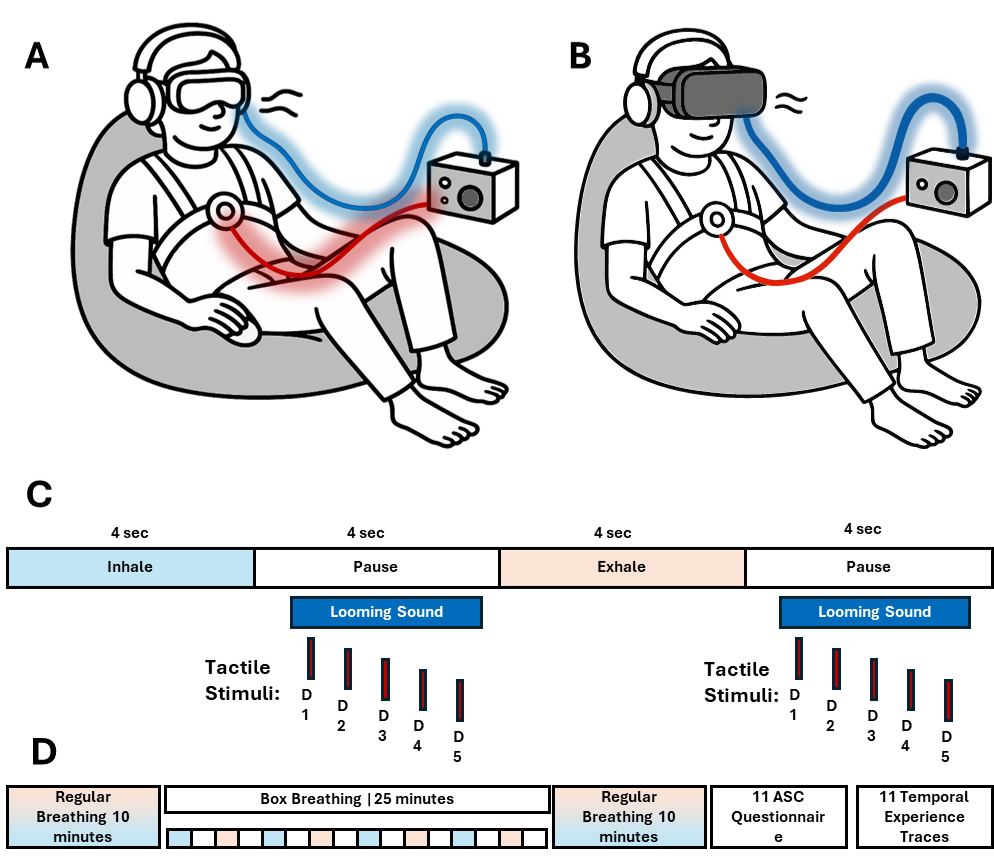
\includegraphics[width=\textwidth]{Fig1.png}
\caption{\textbf{Experimental setup and protocol.} \textbf{A}, Control condition setup with participant wearing headphones (blue cord) and a chest-mounted vibrotactile stimulator (red cord) positioned above the breast area as depicted on the strap itself, providing only the minimal breath-performance feedback indicator without spatial cues. \textbf{B}, Viscereality condition setup with the breath-responsive VR headset providing visual feedback of respiratory state. \textbf{C}, Box-breathing protocol with looming sounds and tactile stimuli presented during breath-hold phases. D1--D5 represent stimulus onset asynchronies between audio and tactile stimuli.}
\label{study5:fig:exp_setup}
\end{figure}

%% ---------------------------------------------------------------------
%% SUBSECTION 1 GOAL
%% One paragraph listing the hardware chain: soundcard, headphones,
%% haptic transducer, respiratory belt, response device, HMD. Ends
%% with the relationship between the two physical outputs of the
%% soundcard and the two transducers reaching the participant.
%% ---------------------------------------------------------------------
\subsection{Apparatus}

%% ---
%% PARAGRAPH GOAL (one idea): enumerate the hardware chain and fix
%% the two-channel output-to-transducer mapping that the rest of
%% the section depends on.
%% ---
Auditory and tactile stimuli were delivered through a Komplete Audio 6 MK2 USB audio interface \citep{komplete_audio_6_mk2}. The audio channel was routed to a pair of Sennheiser HD 560S open-back reference headphones \citep{sennheiser_hd560s}, worn over the ears, and the tactile channel was routed to a Woojer Strap 4 haptic transducer \citep{woojer_strap4}, worn over the chest just above the breast area. Placement was standardised across participants by following the positioning illustration printed on the strap itself, which the operator used as a fitting guide. Participant responses were collected with a standard USB mouse. Respiratory compliance was monitored throughout the session with a chest-mounted respiratory belt transducer positioned around the lower ribcage. In the Viscereality condition, participants additionally wore a head-mounted display delivering the breath-coupled visual environment. In the Control condition, participants viewed the same dark field used as the black-screen control in Study~3, containing only the central breathing performance indicator that scaled with respiratory excursion. This provided minimal feedback stimuli for breath performance without the spatial depth cues, color, or aesthetic properties of the Viscereality environment, and participants did not wear an eye shade (Fig.~\ref{study5:fig:exp_setup}).

%% ---------------------------------------------------------------------
%% SUBSECTION 2 GOAL
%% Describe how the per-participant stereo WAV files were built. Five
%% sub-blocks, one idea per paragraph:
%%   2a  Box-breathing voice guide (pre-recorded MP3).
%%   2b  Looming auditory stimulus (FABIAN HRTF spatialisation).
%%   2c  Tactile pulse (Woojer 4 spec).
%%   2d  Per-trial stereo WAV assembly.
%%   2e  Per-participant sequence construction.
%% ---------------------------------------------------------------------
\subsection{Stimulus generation}
\label{study5:sec:stim_gen}

%% ---
%% PARAGRAPH 2a GOAL (one idea): state that the box-breathing guide
%% is a pre-recorded human-voice MP3 (not a synthesised track), with
%% exact filename, resampling, volume, and channel placement. Keeps
%% the paragraph short and factual.
%% ---
The box-breathing guide was built from two pre-recorded human-voice audio files, one for the inhalation half-cycle and one for the exhalation half-cycle \citep{pydub_audiosegment_note}. Each file voiced a count of ``two, three, four, hold'' over four seconds so that a full 4--4--4--4 cycle of inhalation, post-inhalation hold, exhalation, and post-exhalation hold lasted sixteen seconds. Files were loaded at their source rate and resampled to 44.1~kHz using \texttt{librosa} where available and otherwise \texttt{scipy.signal.resample} \citep{Virtanen2020SciPy, librosa_resample_note}. Amplitude was attenuated to 30\% of source level so that the voice guide remained audible without masking the looming stimuli. The guide occupied the right channel of the per-trial stereo WAV, with the left channel set to silence over the same four-second span.

%% ---
%% PARAGRAPH 2b GOAL (one idea): describe the looming-sound pipeline
%% in enough detail that a reader could reproduce it. Emphasise the
%% FABIAN HRTF source (TU Berlin DepositOnce), the head-diameter and
%% inverse-square scaling, the four counterbalanced noise types,
%% the 110 to 10 cm frontal trajectory at 33.3 cm/s, and the
%% per-trial 500 ms silent padding that fixes the stimulus segment
%% to exactly 4 s.
%% ---
Binaural looming stimuli were initially synthesised from four noise types, namely pink, white, brown, and blue noise; later acquisition versions used a subset, predominantly pink and white \citep{brinkmann2017fabian}. For each noise type, a 3-second trajectory was rendered in which a point source approached the head frontally from 1.1~m to 0.1~m at a constant 33.3~cm/s, at zero azimuth and zero elevation. Source-to-ear distances were computed for an 18~cm interaural distance, and amplitude was scaled by the inverse square of source-to-ear distance. Head-related transfer function filtering used the measured FABIAN head-related impulse response at neutral head-above-torso orientation, specifically the \texttt{FABIAN\_HRIR\_measured\_HATO\_0.sofa} file from the FABIAN database hosted on the Technische Universit\"at Berlin DepositOnce repository \citep{fabian_database_2017, brinkmann2017fabian}. The SOFA file was parsed with the \texttt{sofar} Python library \citep{sofar_python}, the left and right impulse responses for the azimuth-zero, elevation-zero position were extracted, and each was convolved with the per-channel noise trajectory using \texttt{scipy.signal.fftconvolve} \citep{Virtanen2020SciPy}. Each looming file was normalised to 95\% of maximum amplitude to prevent digital clipping and was padded with 500~ms of silence before and after the 3-second approach, yielding a 4-second stimulus segment.

%% ---
%% PARAGRAPH 2c GOAL (one idea): specify the tactile pulse used for
%% the Woojer Strap 4 transducer. The current generator selects a
%% 50 Hz pure sine at amplitude 1.0 with an instant on/off block
%% envelope for 100 ms, so calibration is tuned to transducer
%% resonance rather than to perceptual thresholding.
%% ---
Tactile pulses were generated for the Woojer Strap 4 transducer, whose resonance is near 50~Hz. Each pulse was a 100~ms pure-tone 50~Hz sine at digital amplitude 1.0 with an instant-on, instant-off block envelope, chosen to deliver the maximum mechanical impulse the transducer supports \citep{woojer_strap4}. The stimulus-generation scripts can instantiate pulses at 0, 300, 800, 1500, 2200, and 2700~ms after looming onset, with the 0~ms file serving as an audio--tactile simultaneity stimulus. The participant master blocks used the five non-zero PPS SOAs, namely 300, 800, 1500, 2200, and 2700~ms, so that tactile cues sampled the approaching sound after it had begun moving toward the body.

%% ---
%% PARAGRAPH 2d GOAL (one idea): describe how the breathing guide,
%% looming sound, and tactile pulse are combined into a single 8 s
%% stereo WAV. Fixing the channel layout here matters because the
%% delivery section in Subsection 4 refers back to it.
%% ---
Each trial was compiled as an 8-second stereo WAV file at 44.1~kHz in 32-bit float using \texttt{soundfile} \citep{sounddevice_python}. The file contained a 4-second breathing-guide segment followed by a 4-second stimulus segment. Within the stimulus segment, the looming noise occupied the right channel and the tactile pulse occupied the left channel, positioned at the trial-specific SOA within the 4-second window. Baseline trials carried the tactile pulse without a looming sound, and catch trials carried the looming sound without a tactile pulse. Total trial duration was verified at assembly to within one millisecond of the 352{,}800-sample target.

Source-timing inspection revealed a qualification to the nominal cue schedule. In 167 hash-verified original block recordings from 14 cleared participants, tactile pulses were matched to the archived played-order CSVs; all block-median Audio--Tactile tactile cues occurred 500~ms later within the eight-second trial than Baseline cues with the same nominal SOA label. An independently decoded session from a fifteenth cleared participant showed the same block-median offset in all 12 comparable blocks. The archived generator loads looming inputs already padded by 500~ms and has a path that prepends another 500~ms to assembled Audio--Tactile trials while Baseline trials receive one prepend. This shifts absolute cue time while preserving the within-trial auditory-to-tactile SOA, verified directly where both onsets were decoded in the independent session. The other 25 cleared participants lack comparable cue-time verification, so shared nominal labels cannot establish matched absolute timing across trial types in the full cohort.

%% ---
%% PARAGRAPH 2e GOAL (one idea): describe the three-level randomisation
%% logic: macro-structure preservation, within-block randomisation, and
%% block-order randomisation, including the acknowledged predictability
%% imposed by the 4-4-4-4 rhythm and the mitigation strategies adopted.
%% ---
Per-participant trial sequences were generated under a three-level randomisation logic intended to preserve the planned design at the session level while limiting trial-to-trial predictability within a block. At the macro level, the Condition $\times$ respiratory Phase $\times$ five-SOA grid for Audio--Tactile trials and the trial-type counts were fixed across full sessions. Available noise types varied by acquisition version, so sound-type balance was version-specific rather than common to every participant. Within each block, trial order was drawn from a Gellermann-inspired constrained randomisation in which post-inhalation and post-exhalation trials were interleaved, with the algorithm rejecting any sequence that placed more than three consecutive trials of the same type or distributed a trial type asymmetrically across the two halves of a block \citep{gellermann_1933}. Each session was organised as two parts of six blocks each (12 blocks in total), with the six blocks within each part labelled a through f, and each participant was assigned one block-order permutation drawn from the 720 orderings of the six block labels, applied within both parts. This block-order randomisation distributes any block-level position effects across participants without disturbing the within-block constraints. Each block was concatenated into a single continuous WAV of the stimulus-delivery length, accompanied by a trial-order CSV that recorded the trial type, SOA, noise type, and respiratory phase per trial.

A residual source of predictability is unavoidable in this design. The 4--4--4--4 box-breathing rhythm fixes the within-cycle position of the breath-hold phases at which stimuli can be delivered, so participants can in principle anticipate \emph{when}, within each respiratory cycle, an audio--tactile event might arrive. Removing this regularity is not feasible, because a stable respiratory cycle is the precondition for systematically assessing inhale versus exhale as a test variable; an irregular cycle would compromise phase assignment, which is the central manipulation of the study. We therefore adopted the regular 4--4--4--4 rhythm and limited predictability by other means. \emph{Which} stimulus arrives was randomised across the noise types available in each acquisition version. \emph{Whether} a tactile pulse arrives at all was randomised through the inclusion of catch trials (sound-only, no vibration), which required response inhibition. Together with the within-block constrained randomisation and the per-participant block-order permutation, these manipulations limited cues that a participant could exploit to anticipate any individual trial.

%% ---------------------------------------------------------------------
%% SUBSECTION 3 GOAL
%% One paragraph summarising the within-subjects trial design, trial
%% type proportions, total N per session, and session duration. Cross-
%% references to the trial-design figure.
%% ---------------------------------------------------------------------
\subsection{Trial design}

%% ---
%% PARAGRAPH GOAL (one idea): give the reader the per-session counts
%% and durations so the rest of the methods have scale.
%% ---
The experiment used a within-subjects design adapted from the protocol used to test PPS modulation by vestibular stimulation \citep{pfeiffer2018vestibular}, modified for scheduled audio--tactile measurement during box breathing. Each full session planned 408 trials, organised into two parts of six blocks each (12 blocks of 34 trials), with 240 Audio--Tactile trials, 120 Baseline trials, and 48 Catch trials. Audio--Tactile trials delivered a looming sound followed by a tactile pulse at one of five SOAs (300, 800, 1500, 2200, and 2700~ms; \citealt{lee2021altered, mine2022adaptation, teneggi2013social}). The initial acquisition version used blue, brown, pink, and white spectral noise; later versions predominantly used pink and white, the two sound types present across the whole publication cohort. Within each version, Audio--Tactile trials were planned across the 2 (respiratory phase) $\times$ 5 (SOA) design grid at 24 trials per phase $\times$ SOA cell. Baseline trials delivered only the tactile pulse, used the same five nominal delay labels, and were balanced across respiratory phase (60 inhale, 60 exhale). They provide a tactile-only response reference but have no auditory distance; their absolute cue timing cannot be presumed equal to Audio--Tactile trials at the same label. Catch trials delivered only the looming sound and required response inhibition (48 planned trials), yielding a planned catch rate of approximately 12\%. Each trial lasted 8 seconds, so a full 408-trial session took approximately 54 minutes of stimulus time excluding block-level breaks and instructions (Fig.~\ref{study5:fig:trial_design}). One included session ended before all 408 planned trials had been observed; its missing slots and an exclusion sensitivity are documented in the Results.

\begin{figure}[ht]
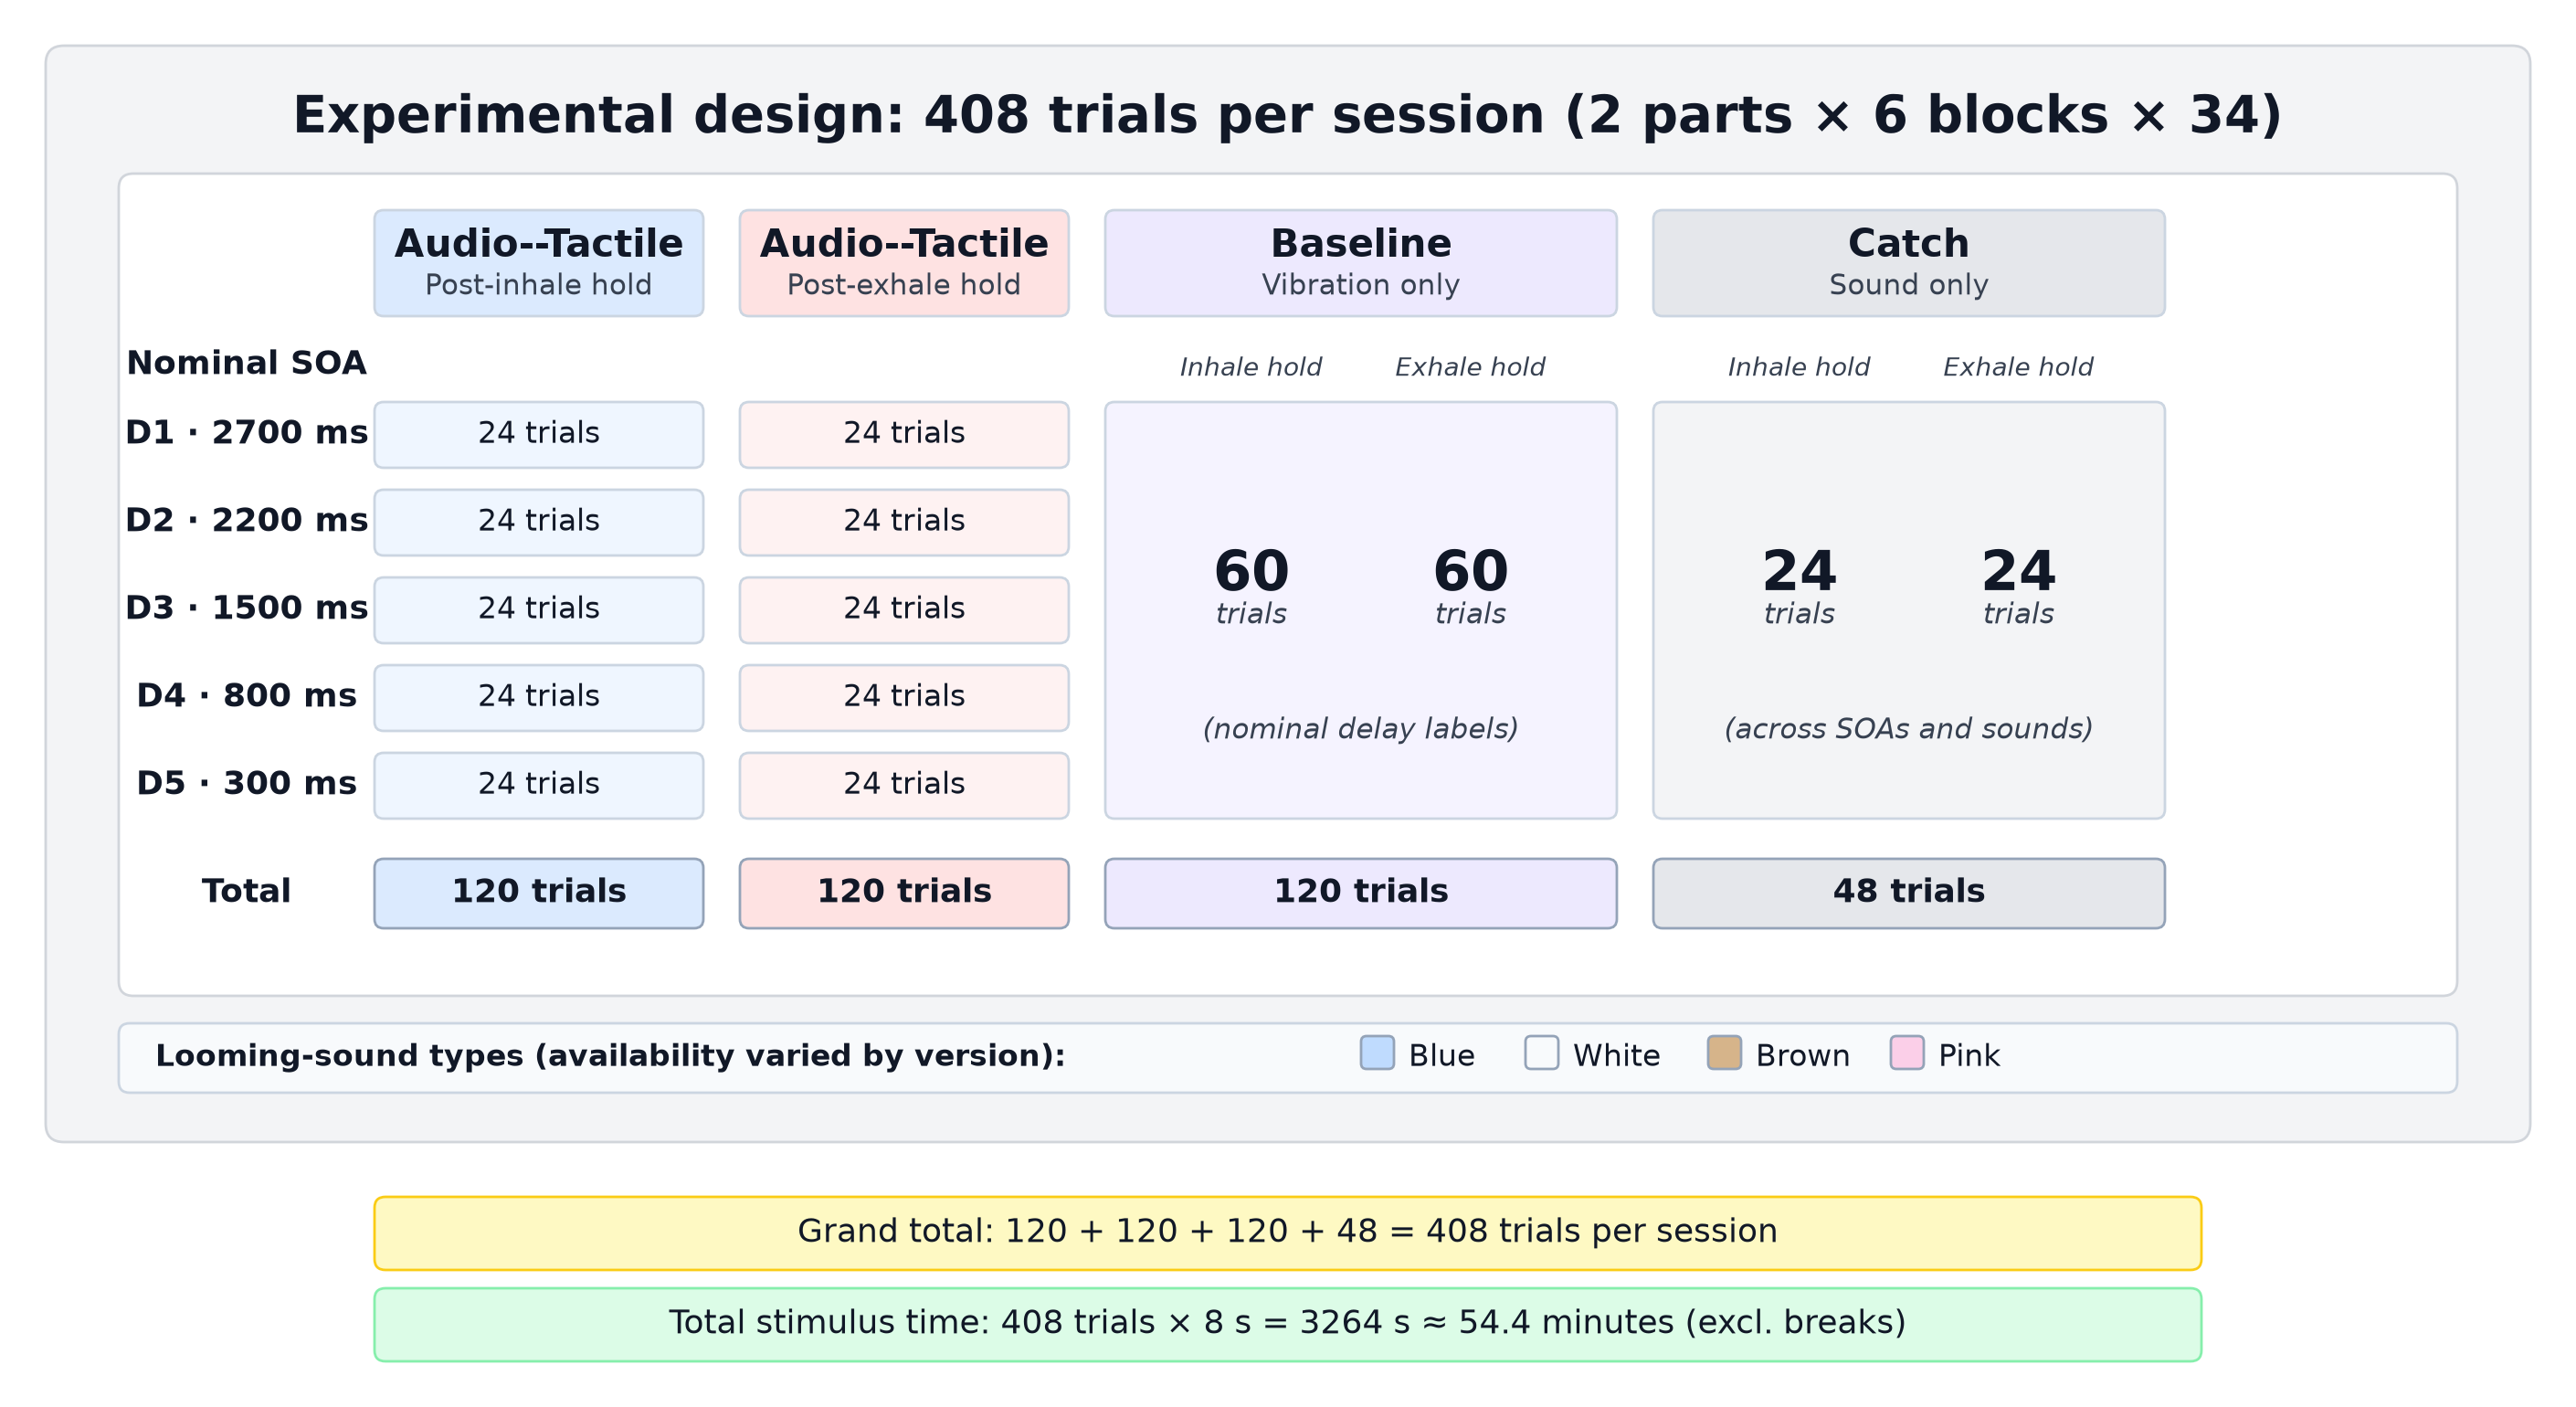
\includegraphics[width=\textwidth]{trial_design.png}
\caption{\textbf{Planned per-session trial distribution across conditions, respiratory phases, and stimulus onset asynchronies.} A full session plans 408 trials, organised as two parts of six blocks (12 blocks of 34). Audio--Tactile trials are distributed evenly across five SOAs (D1--D5; 24 trials per phase $\times$ SOA cell). Available noise types differ by acquisition version. Baseline trials have no auditory SOA or distance; they carry the same five nominal delay labels and are balanced across respiratory phase. Catch trials are balanced across phase and distributed across SOAs and the available noise types.}
\label{study5:fig:trial_design}
\end{figure}

%% ---------------------------------------------------------------------
%% SUBSECTION 4 GOAL
%% Describe stimulus delivery and response capture at run time.
%% Three paragraphs, three ideas:
%%   4a  Playback pipeline and channel routing.
%%   4b  Response capture via a click tone onto the tactile channel.
%%   4c  WASAPI loopback recording of both outputs.
%% The loopback recording is the methodological component that
%% Subsection 5 decodes.
%% ---------------------------------------------------------------------
\subsection{Stimulus delivery and response capture}

%% ---
%% PARAGRAPH 4a GOAL (one idea): how the per-block WAV reaches the
%% participant. Two-channel output, sounddevice callback, WASAPI
%% driver, and the channel-swap that maps file-left to Output 2
%% (Woojer) and file-right to Output 1 (headphones).
%% ---
At run time, each per-block WAV was fully pre-loaded into memory and streamed to the Komplete Audio 6 MK2 on WASAPI via the \texttt{sounddevice} Python binding to the PortAudio library \citep{sounddevice_python}, with a 4096-sample callback block size and a target output latency of 100~ms for stable long-block playback. Python swapped the two channels at the callback boundary so that the left channel of the file was sent to physical Output 2, wired to the Woojer Strap 4 haptic transducer, and the right channel of the file was sent to physical Output 1, wired to the Sennheiser HD 560S headphones. The audio and tactile streams originated from the same file and passed through the same stereo callback, preserving their sample alignment in the digital output stream. Relative acoustic and mechanical onset latencies at the participant were not independently measured.

%% ---
%% PARAGRAPH 4b GOAL (one idea): response capture via click-tone
%% feedback. Each mouse click triggers a short synthetic tone on the
%% tactile channel. The tone is audible to the participant and is
%% what the offline analysis detects, not the OS-level mouse event.
%% ---
Mouse clicks were monitored with the \texttt{pynput} library \citep{pynput_python}, and each click triggered a 1200~Hz, 50~ms synthetic click tone on a separate low-latency \texttt{sounddevice} stream that was routed only to Output 2. The click tone served two purposes. It provided the participant with immediate auditory feedback that the response had registered, and it inserted a detectable event onto the tactile channel that was captured in the loopback recording described below and used for post-hoc reaction-time estimation.

%% ---
%% PARAGRAPH 4c GOAL (one idea): the validated output profile, the
%% continuous WASAPI loopback recording that captures exactly what was
%% sent to the soundcard outputs, and the live event CSV that provides
%% an online behavioural record.
%% ---
Before participant playback, the selected stereo output profile was required to pass a routing preflight in which calibration pulses were sent separately to Output~1 and Output~2 and verified through the corresponding WASAPI loopback endpoint. The documented acquisition profile used the Komplete Audio 6 MK2, with Output~1 assigned to the headphones and Output~2 assigned to the tactile transducer, but the same software could be run on another wired two-channel interface only after the same channel-separation preflight passed. Once participant playback began, the acquisition software was designed to mirror both physical outputs to a WASAPI loopback device and capture them through the \texttt{PyAudioWPatch} extension of the PortAudio interface \citep{pyaudiowpatch}. These source recordings are not presently linked and independently checked for every dataset in the publication pool. Available session WAV files and behavioural CSVs were written to participant-specific data folders with identifying metadata; only coded participant IDs appear in analysis outputs.

%% ---------------------------------------------------------------------
%% SUBSECTION 5 GOAL
%% Describe how the loopback recordings are decoded offline to recover
%% per-trial reaction times. Four paragraphs:
%%   5a  Channel-role inference and tactile-cue detection, plus the
%%       8 s trial grid fit.
%%   5b  Looming onset identification via cross-correlation.
%%   5c  Click-tone detection and RT calculation.
%%   5d  Outcome labelling and alignment to the trial-order CSV.
%% ---------------------------------------------------------------------
\subsection{Reaction-time reconstruction from loopback recordings}

%% ---
%% PARAGRAPH 5a GOAL (one idea): the preprocessing step that turns a
%% continuous loopback recording into a set of per-trial tactile-cue
%% onsets, anchored to an 8 s trial grid. This is the scaffold that
%% every later detection hangs off.
%% ---
For the loopback data to which the waveform-decoding pipeline was applied, reaction times were reconstructed in Python using \texttt{numpy} and \texttt{scipy} \citep{Virtanen2020SciPy}. In that pipeline, audio and tactile channels were identified by the ratio of mean absolute amplitude to root-mean-square amplitude, with the sparser channel assigned as tactile. Tactile cue events were then detected by smoothing the absolute tactile signal with a 10~ms rectangular envelope and thresholding at 0.45 of the envelope peak, subject to a minimum run of 60~ms and a minimum peak amplitude. The resulting cue-onset train was fitted to an 8-second trial grid by jointly minimising the median absolute error between detected onsets and the nominal SOA set, yielding a per-trial cue-onset time in the sample domain of the recorded WAV.

%% ---
%% PARAGRAPH 5b GOAL (one idea): looming onset detection via
%% cross-correlation with the four noise-type templates. This is
%% what lets us label each trial with the noise type actually
%% played and get a second independent anchor for trial timing.
%% ---
For each trial processed by that pipeline, the candidate looming templates for its acquisition version were trimmed to their first 1.5~s of non-silent content, downsampled fivefold for speed, and z-standardised. Each template was cross-correlated with the audio channel of the recording inside the 4.45~s to 7.85~s window relative to the trial origin, using frequency-domain convolution \citep{Virtanen2020SciPy}. The highest-scoring template above threshold assigned the trial its observed noise type and returned the template-onset timestamp, giving an independent anchor for SOA verification where such recording evidence was available.

%% ---
%% PARAGRAPH 5c GOAL (one idea): click-tone detection and RT
%% calculation. The click tone is the actual response event in the
%% recording, and RT is the latency from cue onset to click onset.
%% Emphasises that response timing is measured in the same sample
%% domain as the stimulus.
%% ---
Where the loopback recording and both event markers were available, the 1200~Hz, 50~ms click tone template was z-standardised and cross-correlated with the tactile channel starting at each detected cue onset. Click events were accepted when the local correlation peak exceeded a dynamic threshold of eight median absolute deviations above the local median and were separated from any prior click by at least 100~ms. For such recordings, reaction time was the sample-domain difference between click-tone onset and tactile-cue onset, converted to milliseconds at 44{,}100~Hz. The pooled publication dataset also contains source-recorded reaction times from acquisition versions for which this exact waveform-based definition has not been independently re-harmonised. Consequently the sample-domain timing advantage cannot be assumed for every pooled trial; source-specific timing definitions and verification status are retained in the private provenance crosswalk.

An earlier 40-person source audit catalogued original-recording origins for 31 participants and verified at least one asset hash for each of 17 early-version sessions. That historical audit documented RT-onset variants and unavailable original assets; it is not a new audit of the released 42-person cohort. Source dates, waveform verification status, and acquisition-version identities are deliberately absent from the public tables. The browser companion therefore reports the limits of source-recorded RTs without reconstructing private provenance from arbitrary participant IDs. A file hash establishes source identity, not waveform remeasurement or respiratory-phase accuracy.

%% ---
%% PARAGRAPH 5d GOAL (one idea): outcome labelling and alignment to
%% the per-participant trial-order CSV, producing the analysable
%% dataset. Final sentence returns the reader to the scientific
%% level of abstraction.
%% ---
Trials were labelled against their scheduled trial order and, where available, checked against runtime and recording evidence. Audio--Tactile and Baseline trials with a detected response were labelled hits; Catch trials with a response were false alarms. Unobserved planned slots were kept explicit in the participant audit tables and excluded from reaction-time analysis. Hit-labelled trials without a recorded reaction time contributed to response-quality summaries but not to reaction-time models; missing reaction times were not imputed. The publication-pool analysis table contains only observed planned trials, with trial type, SOA, noise type, scheduled respiratory phase, condition, response outcome, and source-recorded reaction time. Event-marker availability and source location are recorded separately; the analysis table does not imply that every reaction time was newly decoded from a common waveform.

%% ---------------------------------------------------------------------
%% SUBSECTION 6 GOAL
%% Describe how the trial-wise RT table becomes a PPS measure.
%% ---------------------------------------------------------------------
\subsection{Peripersonal-space quantification}

Peripersonal space was operationalised as SOA-dependent audio--tactile reaction time in a looming-sound tactile-detection paradigm \citep{canzoneri2012dynamic, teneggi2013social, noel2015peripersonal}. The tactile pulse occurred at one of five nominal SOAs (300, 800, 1500, 2200, or 2700~ms); longer SOAs corresponded to nearer nominal source positions. The registration labels these SOAs as approximately 100, 73, 50, 27, and 10~cm, although its stated linear 110-to-10~cm, three-second trajectory instead implies approximately 100, 83, 60, 37, and 20~cm at those times. The primary predictor was therefore nominal SOA in milliseconds, not an inferred physical distance. The browser sigmoid implementation retains the registered distance labels for its viability gate; a sensitivity repeated that gate using trajectory-implied positions. It subtracts mean tactile-only Baseline reaction time within each participant $\times$ Condition $\times$ Phase cell: $\mathrm{RT}_{\mathrm{AT}}-\mathrm{RT}_{\mathrm{baseline}}$, with negative values indicating faster Audio--Tactile responses. Baseline trials have no auditory stimulus or acoustic distance. We also compared Audio--Tactile and Baseline RTs at the same nominal SOA label descriptively, without treating the labels as proof of equal cue time. Misses, Catch outcomes, and unobserved planned slots were retained for quality summaries but did not supply reaction times to these curves.

%% ---------------------------------------------------------------------
%% SUBSECTION 6B GOAL
%% Statistical analysis: hierarchical pipeline, sigmoid viability test,
%% model selection, mixed models, ANOVA, contrasts.
%% ---------------------------------------------------------------------
\subsection{Questionnaire scoring and exploratory analysis}

The released participant table contains one set of 37 MAIA-2 items and paired Control/Viscereality spatial-frame-of-reference ratings. The project owner confirmed that MAIA-2 was completed once before the experiment and spatial-frame ratings after each intervention; this timing is supplied by the owner rather than reconstructed from CSV timestamps. MAIA-2 assesses eight self-reported interoceptive dimensions \citep{Mehling2012,Mehling2018}; such reports should be distinguished from objective interoceptive accuracy and metacognitive awareness \citep{Garfinkel2015}. Scores on the administered 0--5 response scale were independently recomputed using the final MAIA-2 item map: Noticing, items 1--4; Not-Distracting, 5--10; Not-Worrying, 11--15; Attention Regulation, 16--22; Emotional Awareness, 23--27; Self-Regulation, 28--31; Body Listening, 32--34; and Trusting, 35--37. Items 5--10, 11, 12 and 15 were reversed as $5-\mathrm{response}$. Each subscale required all constituent items; missing responses were not imputed and no total score was formed. Recomputed and stored means were compared within $10^{-6}$. The release does not supply the administered language record, repeated MAIA scores, or separate body-boundary and small-self fields.

This questionnaire extension is post hoc. Its scoring, estimands and test family were recorded before computing the new associations, but after inspecting the dataset and prior behavioural results. The original registration endpoint returned HTTP 403 during this review; its exact questionnaire wording could not be independently checked. The current repository Methods and analysis contract supply the available account of the plan, with the distinction between registered behavioural questions and this exploratory extension retained. The original registration and administered instrument records require verification before submission.

We reported item frequencies, missingness, subscale descriptives, corrected item--rest correlations and raw Cronbach alpha. Sample-specific reliability can differ by dimension and occasion \citep{Eggart2021}; alpha also has restrictive assumptions \citep{McNeish2018}. We therefore reported pointwise percentile 95\% intervals from 2,000 whole-participant bootstrap draws for means and alpha, without treating a cutoff as evidence of validity, deleting items, or fitting a new 37-item factor structure in this small sample. No clinical change thresholds or pre/post tests were transferred from external validation studies.

Spatial-frame ratings are relevant to experiential changes studied in mindfulness research \citep{hanley_2020}, but the present release includes only condition-labelled A--H responses and corresponding codes 1--8. We verified agreement of these encodings and retained their ordinal order. Category distributions and the full paired transition table were reported. A two-sided exact binomial sign test compared higher versus lower Viscereality ratings among non-ties, with a Clopper--Pearson interval for the higher-rating proportion. Ties remained in the overall paired denominator and in paired dominance, defined as $(n_{\mathrm{higher}}-n_{\mathrm{lower}})/n_{\mathrm{pairs}}$, with a participant-bootstrap interval. Order-stratified counts were descriptive. Equal spacing of categories was not assumed. Because the administered pictogram key is unavailable, higher codes were not labelled allocentric.

The retained supplementary association set comprised 33 Spearman correlations: eight MAIA-2 dimensions with each of Control rating, Viscereality rating, rating-change direction ($-1,0,+1$), and the equal-participant raw-RT Condition $\times$ Phase SOA-slope contrast; plus rating-change direction with that behavioural contrast. The slope contrast used the five cell means and primary SOA scaling; it does not estimate a sigmoid boundary. Complete pairs, average ranks, 19,999 pairing permutations, and the absolute-statistic two-sided tail with the plus-one correction supplied $p$ values. All 33 association $p$ values were reported without multiple-testing correction. This reporting choice replaced the initially specified Holm adjustment after inspecting the results; the analyses remain exploratory. The plus-one rule is part of Monte Carlo permutation inference, not adjustment across tests. Pointwise 95\% intervals used 2,000 paired-person bootstrap draws with re-ranking, excluding and counting undefined draws. Legacy resampling used seed 20261116. These intervals are not simultaneous, and permutation inference assumes exchangeable participants under independence without covariate adjustment. The spatial condition comparison formed a separate, single exploratory test family. Inter-subscale correlations were descriptive without further testing. Missing questionnaires never excluded a person from the primary RT cohort; boundary-related correlations retained the original fit gate.

The main spatial follow-up was subsequently specified as the signed numerical difference $\Delta_i=Y_{i,\mathrm{Viscereality}}-Y_{i,\mathrm{Control}}$, regardless of presentation order. These are two post-intervention ratings, not change from a spatial baseline. This exploratory amendment was recorded before computing the new delta analyses but after inspecting the earlier questionnaire results. All eight continuous MAIA-2 dimensions were correlated separately with numerical $\Delta$ using the same permutation and paired-bootstrap procedure, with an independent generator seeded 20261117. One ancillary correlation linked $\Delta$ to the raw-RT SOA-slope interaction. The eight existing direction-only correlations were retained as ordinal sensitivities; the complete earlier set remained supplementary. Numerical subtraction assumes comparable category steps, and ranking the resulting differences does not eliminate that assumption.

Condition $\times$ pre-experiment MAIA moderation was estimated separately for each dimension by OLS regression of participant $\Delta$ on an intercept and mean-centred MAIA. A second specification added centred presentation order (0=Control-first, 1=Viscereality-first). Differencing eliminates participant intercepts; in this complete two-condition design, the MAIA slope tests the corresponding repeated-measures interaction, while the order coefficient represents Condition $\times$ Order. Independent long-format participant-intercept fits verified the equivalence. Slopes are code steps per one MAIA point. Ordinary two-sided $t$ inference used $n-k$ residual degrees of freedom and interaction $F=t^2$ with $(1,n-k)$ degrees of freedom. This inference assumes a linear conditional mean, independent participants and homoskedastic Gaussian errors. HC3 covariance with $t_{n-k}$ tails supplied approximate heteroskedasticity-sensitive intervals and $p$ values. Both specifications and both uncertainty estimates were reported for every dimension, without multiple-testing correction. Maximum leverage and Cook distance were exported; no participant was removed on these diagnostics. Unknown order excludes a record only from the order sensitivity. Baseline MAIA can moderate the condition contrast; its single pre-experiment measurement cannot mediate an intervention-induced change in MAIA. No mediation analysis was fitted, and order adjustment does not establish absence of carryover.

\subsection{Statistical analysis}
\label{study5:sec:stats}

The analysis plan was registered on AsPredicted (\url{https://aspredicted.org/az9f89.pdf}). The browser implementation follows the registered questions as operationalised in this Methods section, with a fixed executable contract in \texttt{workbook/ANALYSIS\_PLAN.md}. It reads the released 42-person participant and trial tables, preserving the participant as the independent repeated-measures unit. Audio--Tactile and Baseline hits with recorded RT are pooled within person to calculate the mean and sample SD; values within mean $\pm$ 2.5 SD, inclusive, enter RT analyses. Participants with Catch false-alarm rate greater than 30\% are excluded; low hit-rate flags are descriptive. A 200-ms lower cutoff is a sensitivity, not an additional primary rule. The partial session is retained primarily, with explicit exclusion sensitivities. Interactive preparation controls do not change this analysis population.

The primary question uses a Gaussian ML mixed model of individual Audio--Tactile RTs, with Condition, instructed Phase, numeric SOA, all interactions, and a participant random intercept. Control/Viscereality and Exhale/Inhale are coded $-.5/+.5$; SOA is centred and divided by its trial-level sample SD. A likelihood-ratio test compares the full model to the identical model without the three-way term. The secondary model tests Phase $\times$ SOA within Control. Five-level SOA coding is a sensitivity because coding was not fully specified in the registration. Random-intercept ML is profiled exactly using participant sufficient statistics and Woodbury identities, including the zero-variance boundary; it is independently checked against native \texttt{statsmodels} ML fits. Model-based normal Wald intervals condition on estimated covariance parameters and are not small-sample-corrected intervals.

Sensitivities include a participant random SOA slope; linear and log-RT regressions with participant-cluster-robust sandwich covariance; equal-participant contrasts of slopes through five SOA means; complete-person $2\times2\times5$ repeated-measures ANOVA with effect-specific Greenhouse--Geisser correction; condition-order subgroup descriptions; participant-cluster-robust binomial hit-probability regression; and RT regression with within-condition trial position and Condition $\times$ Phase-specific time trends. The random-slope covariance is estimated by Cholesky parameterisation with L-BFGS-B and Powell candidates and a zero-slope boundary. Cluster covariance uses the $G/(G-1)\,(n-1)/(n-p)$ correction and normal Wald inference. The participant-slope sign-flip test uses all sign patterns for at most 16 people and otherwise 19{,}999 Monte Carlo draws with seed 20261015. These analyses probe assumptions rather than replace the primary estimand.

The post hoc missing-RT stress tests assign each hit-labelled Audio--Tactile trial lacking an RT its observed participant $\times$ Condition $\times$ Phase $\times$ SOA cell median. Signed shifts of 0, $\pm100$, and $\pm200$~ms are then applied according to the three-way-contrast direction, and the RT trim and primary model are rerun. These scenarios do not impute misses or identify the missingness mechanism.

The boundary analysis requires trial-level sigmoid $R^2\geq .70$ in all four participant Condition $\times$ Phase cells. The registration did not fully specify the four-parameter form, bounds, trial-versus-mean $R^2$, or whether this exclusion also applied to the raw-RT interaction. We explicitly apply it to boundary inference and report the raw-RT interaction for the roster-based cohort. The transparent reimplementation is $f(x)=a+(b-a)\operatorname{expit}((x-m)/s)$, with $a,b\in[-2000,2000]$~ms, midpoint $m$ within the sampled distance range, and width $s\in[.1,200]$~cm, using three starts. These are disclosed computational choices, not recovered historical optimizer settings. Registered approximate distances and trajectory-implied positions are fitted separately, after subtracting the participant Condition/Phase mean Baseline. Trial objectives use exact SOA sufficient statistics. We additionally calculate the saturated five-SOA trial-level $R^2$ ceiling, which bounds any deterministic SOA curve independently of sigmoid bounds. In-sample sigmoid/linear RMSE, five-mean fits, group fits, and parameter-bound hits are descriptive. Four-parameter fits to five means have one residual degree of freedom and cannot rescue failed trial gates. Boundary midpoint/sharpness and related MAIA-2 or pictographic associations require four qualifying, bound-free trial fits per person; otherwise these outcomes are explicitly not estimable.

A separate post hoc extension examined whether one common procedure could describe four group RT profiles with interpretable sigmoid transitions. Audiotactile and related visuotactile work motivates examining distance-dependent transitions \citep{canzoneri2012dynamic,noel2020rapid}, while expectancy-controlled logarithmic patterns and critical experimental evidence make the response form an empirical question \citep{hobeika2019capturing,holmes2020sounds}. This extension addresses group-profile description; it cannot recover participant boundaries that fail the inference gate. Candidate families were developed after inspecting the data and were not registered. Reporting the full finite grid follows the transparency rationale of multiverse analysis \citep{Steegen2016}, without claiming an exhaustive set of reasonable analyses or treating the most sigmoid-looking result as a confirmatory finding.

Kernel local-constant and local-linear regression provide established signal-smoothing estimators \citep{LiRacine2007}, while local weighted regression, curvature regularization, and isotonic projection provide alternative smooth or shape-constrained approximations \citep{Cleveland1979,Wahba1990,Busing2022}. The four-parameter logistic supplies descriptive location and scale parameters \citep{Ritz2019}; whether the measurements identify them is a separate question from whether the curve fits well \citep{Raue2009}. These sources motivate the estimation tools, not particular bandwidths, bounds, or a requirement that PPS observations follow a sigmoid. The companion's miniature literature review maps each choice to supporting and contrary evidence and records the limits of source access.

The extension used the same retained Audio--Tactile trials and five design positions. Within each participant $\times$ Condition $\times$ Phase $\times$ position cell, five extraction methods were considered: arithmetic mean, median, 10\% and 20\% per-tail trimmed means, and 20\% per-tail winsorized means. Winsorization replaces the lowest and highest $\lfloor .2n\rfloor$ values by the adjacent retained order statistics; it does not remove further trials. The resulting cells were averaged with equal participant weights. Robust summaries probe the influence of extreme RTs and cutoff choices \citep{Ratcliff1993}; the specific percentages remain exploratory. Mean, median and winsorized summaries target different summaries of the response distribution, and the midpoint of a curve through group summaries is not generally the mean of individual midpoints. Thirty-two smoothing specifications crossed Gaussian local-constant and local-linear bandwidths, tricube local-linear bandwidths, discrete curvature penalties, isotonic regression, and Gaussian smoothing followed by isotonic projection, including an unsmoothed comparator. Separate versus common widths across the four curves gave $5\times32\times2=320$ pipelines. Tricube smoothing here is a fixed-bandwidth local-linear implementation without robust residual reweighting; the discrete penalty is not an exact cubic smoothing spline. The complete grid is executable in \texttt{descriptive\_sigmoid.py}.

Distances were normalized to $[0,1]$ using the registered 10--100~cm range. Each candidate fitted $a+A\operatorname{expit}((d-m)/s)$ with $A\in[0,500]$~ms, $m\in[10,100]$~cm and $s\in[4.5,90]$~cm. Increasing RT with distance was imposed as a descriptive shape constraint, allowing $A=0$ rather than forcing a nonzero transition. Offset and amplitude were profiled analytically over 61 equally spaced midpoints and 35 geometrically spaced widths. The selected method used a finer 241-by-81 grid. The width floor prevents transitions substantially narrower than the smallest sampled spacing: its 10--90\% span is 19.8~cm, versus a minimum 17-cm gap. These bounds are explicit regularization choices and were expanded in a sensitivity analysis. No display interpolation was treated as an additional observation.

The same fixed six participant folds (seed 20261016) and five omitted positions evaluated every candidate. For each participant fold and position, extraction, group averaging, smoothing and fitting used only the other participants at the other four positions. The predicted held-out value was centered on the training curve's four unsmoothed extracted values; the fixed scoring target was each test participant's raw cell mean at the omitted position minus that participant's raw mean across the other four positions. Squared errors were averaged over participants, groups and held-out positions. This common shape target permits comparison of mean and robust extraction despite their different overall RT levels. The pipeline with minimum RMSE was selected uniformly for all four curves. Constant and linear benchmarks used identical folds and targets. These reused tuning scores do not constitute an independent post-selection test. Evaluation conditions on profiles cleaned beforehand: participant-wide trimming thresholds use all eligible AT and Baseline hit RTs, including the position later omitted from fitting. Thresholds are not shared across people, but this is not end-to-end prospective prediction with preprocessing learned without the omitted position. The target measures relative profile shape, not absolute RT accuracy.

Uncertainty was described with 1{,}000 participant-cluster bootstrap draws (seed 20261017), retaining all four curves and all five positions together within each sampled person and refitting the selected smoother and logistic model \citep{EfronTibshirani1993}. Within-person extraction is deterministic and can be cached before resampling. Pointwise curve bands include flat fits. Midpoint, width and slope percentile intervals condition on nonflat fits and on the selected method; flat fractions and parameter-bound fractions are reported. Method selection is not repeated within this bootstrap. Paired parameter contrasts use the same resamples and receive no confirmatory $p$ values. Fixed trimmed-mean/kernel alternatives, trajectory-implied coordinates, expanded bounds, and the full candidate table expose method dependence. Subtracting a participant/Condition/Phase constant Baseline would only shift these translation-equivariant curves vertically; no same-label cue-time matching was assumed.

An additional exploratory shape audit required at least the fitted 10--90\% transition within the measured range, two observed positions strictly on each side of the midpoint, one observed position within the 20--80\% transition, and maximum deviation from a best-fitting line on a 181-point display grid of at least 5\% of the model's observed-range change. Positive amplitude was required to classify a transition as visible; flat fits remained allowed. These are explicit post hoc display and sampling criteria, not a validated definition of PPS. The same 320 pipelines were rerun on the restricted grid, and all 160 extraction/smoother combinations were also fitted with a line. Constraints use known design coordinates only, including when a position is omitted; no held-out outcome enters smoothing or fitting. Scores are weighted by the number of test participants, with the same raw-mean contrast target for every family.

To reduce the optimism of reporting a tuning minimum as evaluation evidence \citep{VarmaSimon2006}, six outer participant folds (seed 20261026) each repeated full selection among the candidates of each family using five inner participant folds crossed with five omitted positions. The selected pipeline then predicted outer test participants with each target position omitted from fitting. Inner selection uses all five positions from training participants; this evaluates new people at known design locations, rather than generalization to an unseen experimental design. A zero-contrast constant provides a fourth benchmark. Families and thresholds were developed post hoc, and training sets overlap; no significance test treats folds as independent replicates. Nested evaluation does not remove all sampling variability \citep{Varoquaux2017}; small RMSE differences are interpreted descriptively. The restricted family's final estimates also receive 1{,}000 whole-participant bootstrap refits, conditional on its selected method and constraints. For display, each draw and its corresponding extracted data are centered on the mean across the five sampled positions. Centering is an additive shift and preserves curvature. A separate geometry-only figure normalizes fitted amplitudes, with no observations or uncertainty represented on that scale.

As an independent exploratory check on the observations, raw unsmoothed participant means were projected onto three orthonormal contrasts orthogonal to an intercept and distance. One-sample Hotelling $T^2$ tests assess any nonlinear component, under independent participants, multivariate-normal contrasts and nonsingular covariance. The $F(3,n-3)$ transformation was independently checked against \texttt{statsmodels}; Holm correction covers the four curves. This is not a sigmoid-specific test. The PPS literature motivates investigating distance-dependent transitions \citep{canzoneri2012dynamic,noel2020rapid}, but also reports expectancy-sensitive logarithmic patterns \citep{hobeika2019capturing} and methodological concerns about flexible analysis and small effects \citep{holmes2020sounds}. The focused literature review used indexed abstracts for the PPS and validation papers and official software or author sources for implementation references. Full-paper retrieval and current-literature coverage were limited; the companion records exact searches, access levels and source hashes. No source is taken as evidence that this dataset must be sigmoid.

Supplementary paired contrasts cover Baseline Condition, Phase and their interaction, overall Audio--Tactile-minus-Baseline RT, far-minus-near patterns, same-label Baseline comparisons, and pink-minus-white RT. Their ten unadjusted $p$ values are accompanied by Holm-adjusted values for one family. A four-noise Friedman comparison includes only people with all four sounds available, without assigning acquisition-version labels. Paired contrasts have 95\% $t$ intervals; null detections are not equivalence tests. Same-label Baseline subtraction is descriptive because nominal labels do not establish matched tactile-cue times.

The registration named a Cauchy width of 0.707 but did not fully specify mixed-model priors and comparisons. No BIC approximation is presented as a registered mixed-model Bayes factor. Exploratory one-sample/paired Jeffreys--Zellner--Siow factors use a Cauchy $\sqrt{2}/2$ prior on standardized participant contrasts under a normal likelihood \citep{Rouder2009BayesianT}; Shapiro--Wilk diagnostics accompany them. All data-supported computations run in the browser using NumPy/SciPy in Pyodide, with versions, model status, retained data, and source/input/output hashes in the downloadable record. Source-dependent waveform, respiratory-compliance, date, version, and onset-definition checks are marked unavailable when the public CSVs cannot support them.

%% ---------------------------------------------------------------------
%% SUBSECTION 7 GOAL
%% Brief: respiratory compliance monitoring and participants. One
%% paragraph each.
%% ---------------------------------------------------------------------
\subsection{Respiratory compliance and participants}

%% ---
%% PARAGRAPH GOAL (one idea): clarify that the respiratory belt
%% signal is a compliance check, not an online gating signal, because
%% phase assignment is baked into the WAV structure at generation.
%% ---
Respiratory phase was assigned in the trial schedule under the instructed 4--4--4--4 box-breathing pattern; trials were not gated online by the belt signal. The archived decoder identifies which prerecorded breathing instruction played and can reconstruct final phase labels from trial-order parity. These procedures identify the instructed half-cycle, not the participant's measured inhalation or exhalation. A respiratory belt was part of the acquisition protocol, but the current publication-pool trial table contains protocol phase labels rather than independently belt-verified phases. The available source recordings do not yet support a uniform trial-by-trial respiratory-compliance audit across all four acquisition versions. Phase-related effects must therefore be interpreted as effects of instructed phase under the compliance assumption.

%% ---
%% PARAGRAPH GOAL (one idea): participants. Reports the actual N for
%% the analysed batch and flags the order-condition confound that
%% future counterbalanced data are intended to resolve.
%% ---
The released cohort contains 42 adults aged 19--37 years, with 41 complete sessions and one partial session. Each participant was scheduled for both VR conditions, and 21 completed each condition order. The registration disclosed eight already-collected pilot participants and a stopping target of 30 complete datasets, 15 in each order. The released roster exceeds that target; dates and the reason for continued collection cannot be reconstructed from these public CSVs and require author documentation before submission. A balanced pooled order split does not establish balance within historical acquisition versions. One participant has behavioral PPS measures without the questionnaire battery. The project owner confirmed ethical approval and authorised public release of the deidentified data after removal of names and verification of a separate backup; approval-body details should be supplied by the authors for the final ethics statement.

\section{Results}

\subsection{Released cohort and response quality}

The analysis used all 42 participants in the released tables (34 women, 8 men; mean age 23.0 years, SD 4.0, range 19--37). Twenty-one completed each condition order. There were 17{,}114 observed trials of 17{,}136 planned slots: 10{,}068 Audio--Tactile, 5{,}033 Baseline, and 2{,}013 Catch trials. Forty-one sessions were complete; one partial session lacked 22 trials but supplied all 20 Condition $\times$ Phase $\times$ SOA cells. There were 24 Catch false alarms, and no participant exceeded the 30\% Catch exclusion rule. Low-hit-rate flags are reported without adding an exclusion criterion.

Among hit-labelled trials, 105 RTs were missing (80 Audio--Tactile and 25 Baseline). These trials remained in hit-rate denominators. The participant-wide mean $\pm$ 2.5-SD trim removed 382 of 13{,}694 recorded hit RTs, retaining 8{,}916 Audio--Tactile and 4{,}396 Baseline RTs. Adding a 200-ms minimum after trimming removed no further observations. Forty-one participants had the full questionnaire measures and one had PPS measures only.

\subsection{Primary interaction and sensitivity analyses}

Adding the Condition $\times$ Phase $\times$ numeric-SOA term to the trial-level random-intercept ML model did not improve fit, $\chi^{2}(1)=0.024$, $p=.878$. With symmetric Condition/Phase coding and standardized SOA, its estimate was 0.81~ms per SOA SD (SE 5.31; 95\% model-based Wald CI $[-9.60, 11.23]$). This interval permits effects in either direction and does not establish equivalence.

The categorical-SOA comparison gave $\chi^{2}(4)=2.27$, $p=.686$. Excluding the partial session left 41 participants (numeric $p=.807$; categorical $p=.773$). The Control-only Phase $\times$ SOA test was also not detected (numeric $p=.430$; categorical $p=.468$). Allowing a participant random SOA slope yielded $p=.859$. The participant-cell repeated-measures three-way interaction was $F(4,164)=0.99$, Greenhouse--Geisser $\epsilon=0.839$, corrected $p=.406$.

The equal-participant five-SOA slope contrast was 0.03~ms per SOA SD, 95\% CI $[-7.88, 7.95]$, $t(41)=0.008$, $p=.993$. The Monte Carlo sign-flip test used 19{,}999 draws with a fixed seed ($p=.994$). Its exploratory paired JZS factor was $\mathrm{BF}_{10}=0.167$ ($\mathrm{BF}_{01}=6.00$). This normal-likelihood participant model is distinct from the registered mixed model; the slope distribution departed from normality (Shapiro--Wilk $p=.005$).

The exploratory participant-cluster-robust models gave the following three-way terms. Normal Wald intervals use the documented finite-cluster sandwich correction.

\begin{center}
\begin{tabular}{lrrr}
Model & Estimate & 95\% CI & $p$ \\
\hline
Raw RT & -1.543 & $[-9.57, 6.49]$ & $.706$ \\
Log RT & -0.003 & $[-0.01, 0.01]$ & $.614$ \\
Time-on-task-adjusted RT & -1.584 & $[-9.59, 6.42]$ & $.698$ \\
Hit probability (log odds) & 0.001 & $[-0.23, 0.24]$ & $.994$ \\
\end{tabular}
\end{center}

The missing-hit-RT stress tests imputed only the 80 Audio--Tactile hits lacking RTs, then recomputed trimming. Median-only imputation gave $p=.960$; signed $-200$ and $+200$~ms scenarios gave $p=.428$ and $p=.253$, respectively. These specified scenarios do not recover missed-trial RTs or identify the missingness mechanism. Full model coefficients, scaling, diagnostics, intermediate tables, and all stress scenarios are in the companion's downloadable report.

\begin{figure}[htbp]
\centering
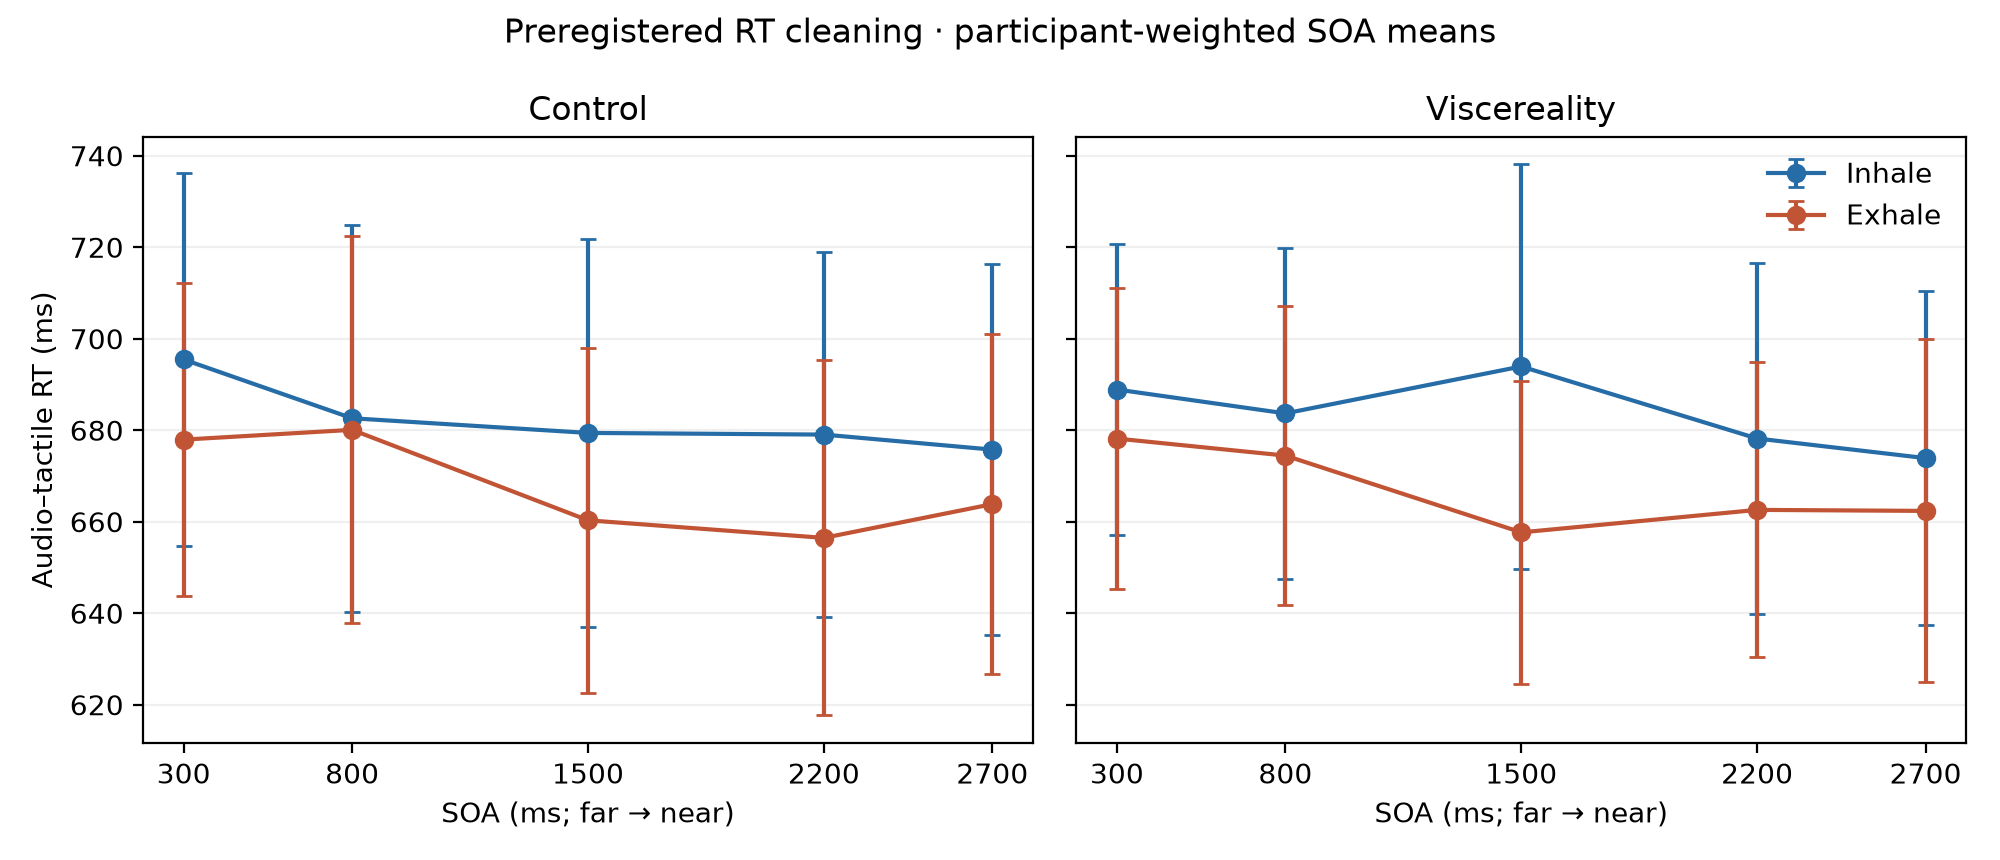
\includegraphics[width=\textwidth]{study5_current_rt_soa_curves.png}
\caption{\textbf{Audio--Tactile RT by SOA, Condition, and instructed respiratory phase in the 42-person cohort.} Each point averages participant means with equal person weight; all cells contain 42 participants. Intervals are pointwise 95\% $t$ intervals across participant means. Longer SOAs correspond to nearer nominal auditory positions. Lines connect means and are not sigmoid fits; inference comes from the stated models.}
\label{study5:fig:current_rt_soa}
\end{figure}

\subsection{Sigmoid viability and descriptive PPS shape}

None of 168 trial-level participant $\times$ Condition $\times$ Phase sigmoid fits reached $R^{2}\geq .70$ (median $R^{2}=0.038$; maximum 0.419). The largest saturated five-SOA trial-level $R^{2}$ ceiling was 0.430. Thus no deterministic sigmoid of these SOAs could reach .70 in any cell, independent of the particular nonlinear optimizer or parameter bounds. Sigmoids improved unpenalized in-sample RMSE over a line in 164/168 cells; this does not establish stable boundaries.

Fitting four parameters to five SOA means instead yielded 79/168 qualifying cells and 3 participants passing all four cells, with none having four bound-free fits. Such fits have one residual degree of freedom and were not used to rescue the failed trial-level gate. Replacing approximate registered distances with trajectory-implied positions left the trial-level pass count at zero. Parameter-bound diagnostics and group fits are supplied descriptively. Participant midpoint/sharpness contrasts and their MAIA-2 or pictographic associations were not estimable under the planned fit gate.

\subsection{Baseline, sound, and order diagnostics}

Across ten supplementary paired contrasts, Holm adjustment was applied as one family. Overall Audio--Tactile minus within-Condition/Phase mean Baseline RT was -18.81~ms, 95\% CI $[-27.00, -10.63]$, unadjusted $p<.001$, Holm $p<.001$. Baseline Inhale minus Exhale RT was 18.08~ms, 95\% CI $[3.28, 32.88]$, unadjusted $p=.018$, Holm $p=.143$. The Baseline Condition $\times$ Phase contrast was 17.43~ms, 95\% CI $[1.56, 33.30]$, unadjusted $p=.032$, Holm $p=.225$. These checks neither establish phase invariance nor provide adjusted evidence of a Baseline phase difference.

The far-minus-near Audio--Tactile difference was 13.80~ms, 95\% CI $[-1.82, 29.42]$; the analogous Baseline nominal-label difference was 11.69~ms, 95\% CI $[-6.90, 30.28]$. Their difference was 2.11~ms, 95\% CI $[-18.44, 22.66]$. Far Audio--Tactile minus Baseline was -10.50~ms using the Condition/Phase reference and -24.83~ms using the same nominal SOA label (Holm $p=.023$ for the latter). Equal labels do not establish cue-time matching; these differences cannot isolate auditory proximity or remove temporal expectancy.

Pink-minus-white Audio--Tactile RT was -2.86~ms, 95\% CI $[-9.30, 3.58]$. Among the 20 participants with all four noise types available, the exploratory Friedman test gave $\chi^{2}(3)=7.80$, $p=.050$. This availability-defined subset cannot be assigned to an acquisition version from the released tables. The two order subgroups each contained 21 participants; their slope contrasts were -4.19~ms, 95\% CI $[-14.64, 6.27]$, and 4.25~ms, 95\% CI $[-8.27, 16.78]$. These descriptive subgroup results do not establish order equivalence.

\begin{figure}[htbp]
\centering
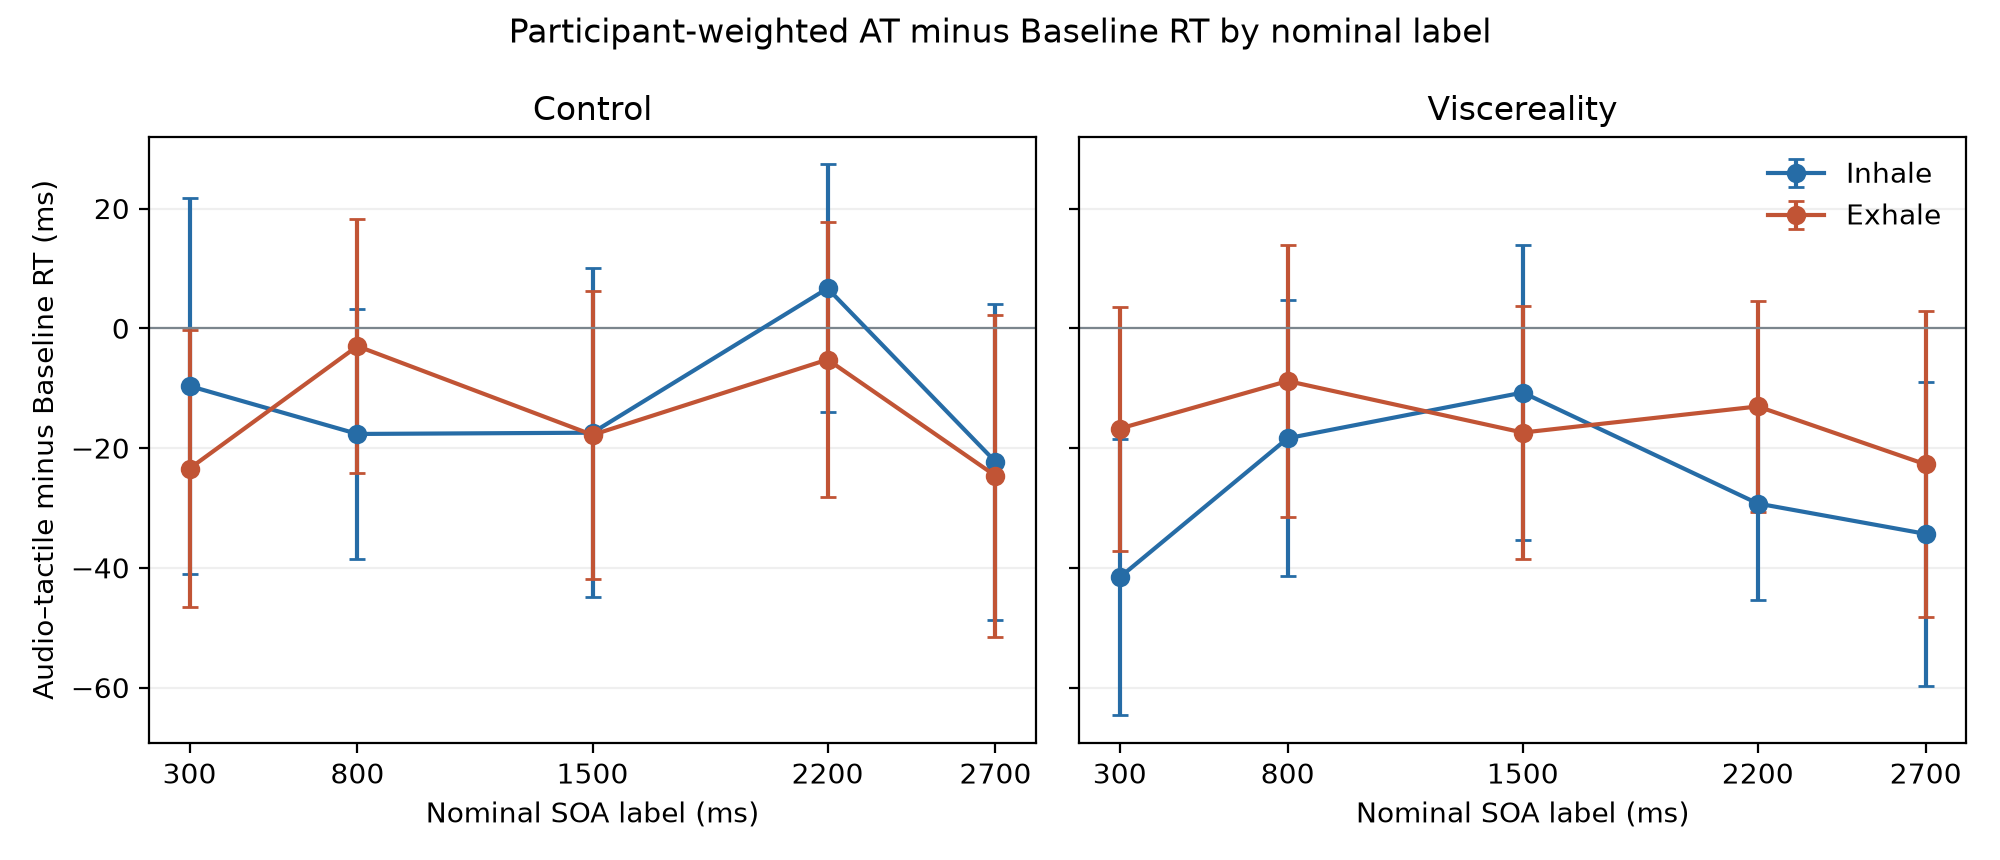
\includegraphics[width=\textwidth]{study5_delay_matched_facilitation.png}
\caption{\textbf{Exploratory Audio--Tactile minus Baseline RT paired by nominal SOA label.} Points average 42 participant differences within Condition $\times$ Phase $\times$ label. Negative values indicate faster Audio--Tactile responses. Baseline has no sound; matching labels does not establish equal trial-relative tactile-cue time. Intervals are pointwise 95\% $t$ intervals across participants. Lines connect means and carry no boundary inference.}
\label{study5:fig:delay_matched_facilitation}
\end{figure}

\subsection{Reproducibility and evidence limits}

All reported behavioral computations were executed in the marimo browser companion with Pyodide, Python 3.14.2, NumPy 2.4.3, SciPy 1.17.1, and Matplotlib 3.10.8. The archived browser download records input, code, and output SHA-256 hashes. Native reference checks independently verified random-intercept ML fits, cluster-robust linear and binomial coefficients/uncertainty, repeated-measures $F$ statistics, and JZS quadrature. A failed or unavailable check is distinguished from a computed null result.

The released CSVs do not contain waveforms, belt recordings, acquisition-version labels, collection dates, or the private provenance needed to identify two historically documented RT-onset variants. The browser analysis therefore does not rerun waveform timing, measured respiratory compliance, pilot-date classification, version-specific contrasts, or that source-definition exclusion. Historical source audits remain historical evidence, rather than new 42-person verification.

\section{Discussion}

The analysis did not detect the predicted Condition $\times$ instructed Phase $\times$ SOA interaction in the released 42-person cohort. Numeric and categorical coding, partial-session exclusion, participant-cluster-robust uncertainty, and equal-participant slopes led to the same qualitative conclusion. The intervals permit effects in either direction, so the result does not establish equivalence or the absence of respiratory influences on PPS.

Audio--Tactile responses were faster than tactile-only responses on average, but neither the raw SOA gradient nor subtraction of Baseline at the same nominal delay label isolates auditory proximity. Historical source checks found unequal trial-relative tactile-cue times for equal labels; the public tables cannot rerun those waveform checks. Temporal expectancy, response probability, trial counts, and control conditions matter when interpreting near-versus-far tactile benefits \citep{holmes2020sounds}. Baseline phase contrasts were uncertain after adjustment across the supplementary family; these data establish neither phase invariance nor an adjusted Baseline phase effect.

The participant-level sigmoid gate failed in every trial cell. The saturated five-SOA ceiling shows that the required trial-level variance explanation is unattainable for any deterministic curve of these SOAs, independently of nonlinear optimizer settings. Better in-sample sigmoid than linear RMSE therefore does not supply valid participant-boundary estimates. Four parameters fitted to five SOA means leave one residual degree of freedom and often meet parameter limits; group curves likewise cannot provide participant replicates. The disagreement between approximate registered distances and the stated trajectory changes some descriptive fit diagnostics but leaves the trial-level gate failure unchanged. Participant-boundary, sharpness, and related questionnaire hypotheses consequently remain unestimated under the planned gate.

The separate descriptive extension did obtain four sigmoid approximations through a uniform signal-extraction and smoothing procedure. Winsorized participant-cell summaries followed by Gaussian-kernel smoothing had the best score among the 320 examined pipelines. The fitted midpoints and slopes permit explicit descriptive comparisons, and all four point estimates were nonflat and inside the specified distance bounds. Their interpretation is nevertheless limited by wide bootstrap intervals, flat resamples, sensitivity to extraction and smoothing, and a small prediction-score gain over a line. Every fitted 10--90\% transition exceeded the sampled distance span. Thus the full S shape and asymptotes are features of the model extrapolation; the study did not observe both plateaus. The bootstrap conditions on the selected method, so it understates total uncertainty if interpreted as including the search itself. A future design with more positions spanning both plateaus, and an independently specified extraction/bandwidth rule, would allow a stronger test of midpoint and sharpness differences.

Several features constrain physiological interpretation. Phase labels identify the instructed half-cycle rather than measured, trial-by-trial belt phase. Historical acquisition sources differ in RT definitions, available sounds, and recording availability; the released CSVs do not identify versions or support uniform waveform harmonisation. The hit-probability and time-on-task checks do not identify RTs on missed trials. The missing-hit-RT scenarios probe specified departures from cell medians and cannot establish the missingness mechanism. The recorded behavioral results should therefore not be read as a precise test of physiologically measured PPS boundaries.

Registration distinctions also require transparent reporting. The Bayesian mixed-model comparison was not fully specified, so the exploratory paired JZS factor addresses a different model and is sensitive to its normal-likelihood assumption. The sigmoid exclusion's scope and computational details required explicit interpretation. The registration disclosed pilot observations, and the released roster exceeds its stopping target; the collection history and ethics-statement details require author documentation before submission. Those items cannot be inferred from arbitrary public participant IDs.

The marimo publication companion makes the data-supported analysis inspectable and executable in the reader's browser. It exposes preprocessing counts, fixed analysis choices, model uncertainty, failed fit gates, unavailable provenance checks, and downloadable source and result hashes. Independent native checks support numerical agreement without substituting precomputed results for browser execution. This reproducibility supports assessment of the reported null detection while preserving the distinction between an executable analysis draft and a paper ready for submission.


\nolinenumbers

\section*{Acknowledgements}
We thank all participants and collaborators who contributed to this research.


\bibliographystyle{apacite}
\bibliography{references}

\end{document}
